
%----------------------------------------------------------------------------------------
%	PACKAGES AND OTHER DOCUMENT CONFIGURATIONS
%----------------------------------------------------------------------------------------

\documentclass[11pt]{article} % Default font size is 12pt, it can be changed here

\usepackage{geometry} % Required to change the page size to A4
\geometry{a4paper, margin=2cm} % Set the page size to be A4 as opposed to the default US Letter

\usepackage{graphicx} % Required for including pictures

\usepackage{float} % Allows putting an [H] in \begin{figure} to specify the exact location of the figure

\usepackage{cite}
\usepackage{amsmath}
\usepackage{gensymb}
\usepackage{url}

\begin{document}
	\begin{titlepage} % Suppresses displaying the page number on the title page and the subsequent page counts as page 1
	
	\raggedleft % Right align the title page
	
	\rule{1pt}{\textheight} % Vertical line
	\hspace{0.05\textwidth} % Whitespace between the vertical line and title page text
	\parbox[b]{0.75\textwidth}{ % Paragraph box for holding the title page text, adjust the width to move the title page left or right on the page
		
		{\Huge\bfseries Reading Project: \\[0.5\baselineskip] Industrial Mathematics}\\[2\baselineskip] % Title
		{\large\textit{Margaret Duff}}\\[3\baselineskip] % Subtitle or further description
		{\large{Semester 1 2018}}\\[3\baselineskip] % Subtitle or further description
		{\Large\textsc{Supervised by: Professor Chris Budd}}\\[4\baselineskip] % Author name, lower case for consistent small caps
		{ABSTRACT}\\[1\baselineskip]
		{This report forms the conclusion of a reading project completed at the University of Bath supervised by Professor Chris Budd. 
			The first part of the report focuses on the International State of Industrial and Applied Mathematics, Mechanisms, Philosophy and Effectiveness and includes four case studies showing just some of the breadth of applicable mathematics research carried out. The second part of the report looks at a specific Industrial Mathematics problem, that of modelling temperature variations due to High Intensity Focused Ultrasound on structures including human muscle and bone. A background to the problem is given, along with examples of previous work before some current work is explained.  }\\[4\baselineskip]			
	}
	
	\end{titlepage}

\pagebreak
	\tableofcontents 
	\pagebreak
	\section{Introduction}
	
	
	Weather and climate prediction, modern slavery, data protection, epidemic modelling, city planning and  plant science are just a small list of the areas of research and policy that are vital for a fast growing 21st Century Population. Underpinning research and decision making in these areas there are mathematicians working on complex PDE systems on a sphere to model the earth's atmosphere; creating dynamic models of plant systems and of epidemic and city growth and  providing image analysis algorithms to capture plant data effectively. There are  statisticians working on providing estimates of the total number of modern day slaves, they are estimating re-arrest rates to give guidance on how long police data should be kept for and dealing with the explosion in complete genome driven by advances in sequencing technology. All of these are examples of the importance of Mathematics to a modern day society.
	 
	
	The project is split roughly in 2 parts. The broad aim for the first part of the project was to: ``Evaluate the  International State of Industrial and Applied Mathematics, Mechanisms, Philosophy and Effectiveness". Some initial and investigation lead to the realisation that the first task, defining what exactly is `industrial mathematics', could have constituted a full project in itself.  Section, \ref{definitions} defines a working definition that will be used throughout the report. 
		Section \ref{significance} then looks at why this is  a topic worth studying before section \ref{current state } looks at the state of Industrial mathematics.  Some common mechanisms for engaging in industrial mathematics are discussed, then the incentives and enablers to engaging in industrial mathematics. Next, in section \ref{SF} the definition of success is considered for industrial mathematics, and examples are given. Finally, section \ref{challenges} looks at the challenges and areas for improvement for the success of industrial mathematics. Problems in selecting suitable problems, building working relationships, the challenges of intellectual property ownership, how industrial mathematics fits into a career path and finally Brexit are discussed. This report will mainly be  focused on the UK but we will look elsewhere in the world for examples and comparisons. 
	
	
	 A report critical to the development of  section 2 was compiled by Professor Philip Bond entitled `The Era of Mathematics: An Independent Review of Knowledge Exchange in the Mathematical Sciences', \cite{Bond}, which was facilitated by the Engineering and Physical Sciences Research Council and the Knowledge Transfer Network. It provides 26 recommendations for government, industry and academia to strengthen and support the role mathematical sciences plays in innovation. In putting together the report a wide range of individuals and institutions were consulted and the report was overseen by an expert review committee. 
	
	Throughout I will reference and draw examples from four case studies included at the end of Section 2 (sections \ref{landmines}, \ref{homeless}, \ref{Milan} and \ref{Africa }) showing just some of the breadth of applicable mathematics research carried out. Choosing just four case studies was very difficult, and there are many many more shining examples of good industrial mathematics. 
	
	Section \ref{extended}, moves on to look in detail at a problem brought to an Industrial Problem Solving Workshop at the Fields Institute in Toronto, by the Hospital for Sick Children in Toronto. The problem looked at modelling the effect of High Intensity Focused Ultrasound (HIFU) on human internal structures. HIFU has applications for cancer therapy through thermal hyperthermia, localised drug delivery and modification of tissues. It is non-invasive so of great interest, especially in paediatric and foetal applications. It is also a challenge mathematically with complex structures and sometimes multiple processes. The report aims to set out some of the background to HIFU before discussing the study group problem, and the progress made during the week. Finally, it looks at some other avenues of research and the current and potentially future work of this project. 
	
	The last section, that of final thoughts, will bring the report together and will attempt to give priority areas for improvement in state and effectiveness of industrial mathematics over the next few years. 
	
	\pagebreak
	\section{Review of the International State of Industrial and Applied Mathematics, Mechanisms, Philosophy and Effectiveness}
	

	
	\subsection{Definitions \label{definitions} }
	
	Defining the language and descriptors of  Industrial Maths is not a simple task and indeed a variety of distinguished writers choose a range of definitions. 
	
	Even defining what it means to do Mathematical Research is fraught with complications. Counting all those employed by universities and higher education institutes misses a large number of very talented mathematicians working elsewhere. 	Deloitte in their report `Measuring the Economic Benefits of Mathematical Science Research in the UK' \cite{deloitteuk} count `Mathematical Science Occupations' as those `which either entail mathematical science research, or used mathematical science research-derived tools and techniques' a broad definition which includes individuals which may use mathematically derived techniques but have no understanding of the underlying mathematics. For example they include: all hospital and healthcare managers, social science researchers and public service administrative professionals, all very valuable jobs but not ones that I would put in the category of `Mathematical Science Occupations'. 
	
	
	In a similar report Deloitte produced for the Dutch economy \cite{deloitteNL} they narrow this definition slightly by considering `only people in jobs requiring a higher education' to be included.  A better but still quite broad definition and probably still includes healthcare managers and social science researchers!
	
	
	One might suggest considering only those people who currently use or research `modern' mathematical science research tools, to avoid including all those people that use an excel spreadsheet to add up large numbers because ``addition" is a mathematical technique. But then the definition of `modern' is fraught: number theory developed during the end 19th and beginning of the 20th century underpins the very modern phenomenon of internet shopping. The radon transform, also developed at the beginning of the 20th century, is behind most modern medical imaging. The motion of a rocket from the surface of the Earth to a landing on the Moon can be explained and described by physical principals discovered over 300 years ago by Sir Isaac Newton.
	
	
	For the purpose of this report, I  will consider Mathematics to be that which is of interest to academic mathematicians; it focuses  on the underlying structure and pattern of a problem and  looks for generalisations and derives exact or approximate solutions backed up by logical proof. The important clarification is that the application of well known techniques does not count finally discounting those Social Scientists using statistical software)!
	
	
 Industry,  I define to be any non-mathematical institution including: governments, businesses, manufacturers, other academic departments, hospitals, schools, charities etc. 


		A wealth of words are used as synonyms or colloquialisms for industrial mathematics: `applicable', `interdisciplinary, `applied', `knowledge transfer' or `mathematics communication'. The Bond Report \cite{Bond} describes `\textit{Impactful Mathematics} as any mathematical method that has practical application and generates societal and/or economic value'. 
		
		For this report I will use the definition John Stockie describes in his essay `Mathematics for Industry a Personal Perspective' \cite{Stockie2015} that Industrial Mathematics includes: 
		
	\begin{itemize}
	\item mathematics that is done by non-academic mathematicians who work as employee of a company
	\item mathematics that is done by academic mathematicians within research institutions for a company, or in collaboration with a company
	\item mathematics that is inspired by industry and arise from an industrial setting. 
	\end{itemize}
	
	
	\subsection{Significance \label{significance}}
	
Although most people don't grow up to become mathematicians, they do grow up to rely on mathematics: from weather forecasts to smart phones; from the logistics of ensuring fresh food in supermarkets to online shopping or from the mechanics of a car engine to  the ability to understand the mysteries of the universe. Mathematicians like to tell you that ``Maths is Everywhere" and indeed it is! 

However, a more quantitative argument, of why Mathematics is important, is required to convince the most sceptical of readers. The Deloitte Report on the Economic benefits of mathematical research on the UK economy \cite{deloitteuk}, although perhaps over estimating as discussed above, suggests that a total of 9.8 million people are in employment attributed to mathematical science research. This can be further broken down into: 2.8 million  directly attributed to mathematical science research, 2.9 million employed indirectly through `supply chain' impacts e.g. support staff, cleaners and technicians and finally 4.1 million people have employment induced  through spending by households linked to mathematical science research. They also concluded that in 2010, mathematical science research in the UK generated direct gross-value added (GVA, value of the output less the value of the immediate consumption) of approximately £208 billion, or around 16\% of total UK GVA.  Productivity, GVA per worker, in Mathematical Science occupations in 2010 was calculated at £74,000 per worker which can be compared to the UK productivity average in 2010 which was estimated to be £36,000 and the mean wage for mathematical science research jobs at over £44,000. 
 
 Similar work by Deloitte on analysis the Dutch economy \cite{deloitteNL} came up with Mathematical Science contributing 9.5\% of total GVA and the GVA per job is 77,000 Euro, 21\% above the national average. With the slight differences in the  definitions of mathematical science jobs between the two reports, I don't think these values can be directly compared. The results of both reports, however,  highlight the significance of Mathematical Science Research on developed economies and therefore how important that the UK ensures it continues to grow and remain competitive.
 
 
	
	 
	\subsection{Current State \label{current state }}
	
	\subsubsection{ Mechanisms in the UK  }
	This section aims to list just some of the avenues for companies and academics in the UK to pursue collaborations, it is in no way a complete list. The Bond report \cite{Bond} found from its call for evidence a list of the most commonly cited examples of industrial mathematics mechanisms. This included: 
	\begin{itemize}
		\item \textit{Industrial Cooperative Awards in Science and Technology (CASE) PhD studentships } are to fund PhD projects in industrial mathematics.  A company allocated an award defines a research project and picks an academic partner. Once the arrangements for the project have been agreed between the company and research organisation, they can recruit a student. Students receive funding for a full EPSRC studentship for 4 years topped up by the company. A placement of at least 3 months at the company is required and projects should be in the area of engineering and the physical sciences. Students benefit from access training, facilities and expertise not available in an academic setting alone and academic partner institutions benefit from novel research collaborations and  development/ strengthening  of partnerships. 
		Companies that were awarded EPSRC ICASE allocations for 2019/20 include the Defence Science and Technology Laboratory, Rolls-Royce PLC and the National Physical Laboratory \cite{CASE}.  
		
		\item \textit{Knowledge Transfer Network Ltd activities } are funded by Innovate UK  and provides innovation network for other funders in line with its mission to drive UK growth. Examples of their programmes include: 
		\begin{itemize}
			\item \textit{ The 4manufacturing initiative } provides strategies for businesses to identify their barriers, challenges and next steps on the path to integrating modern technologies and systems to use digital data within both the business and the supply chain
			\item \textit{Knowledge transfer partnerships} (see below )
			\item \textit{Special Interest Groups} projects that focus our activity and accelerate innovation in cross-disciplinary topics of strategic importance. Groups funded included: Sustainable Aviation Fuel, Synthetic Biology, and Uncertainty Quantification and Management.
			\item \textit{The Access to Funding and Finance team} can help businesses understand and raise funding and finance – lending, grants, or equity based, as well helping prepare companies for investment.
		\end{itemize}
		\item \textit{Mathematics Study Groups} - Provide a forum for industrial scientists to work alongside academic mathematicians  on problems of direct industrial relevance. Initiated in Oxford in 1968 the format has been copied around the world and in even extending into other areas. The structure is as followed: 
		\begin{itemize}
			\item Approximately 80 mathematicians from a wide range of backgrounds
			\item On the first day the industrial representatives outline their project and aims
			\item The following few days are devoted to solving the problems. The industrial representatives are available to answer questions and guide the projects.
			\item On the last day, any progress made is presented
			\item Reports in the problems are produced after the meeting  
		\end{itemize}
		There are many benefits to industry including: 
		\begin{itemize}
			\item Access to the expertise of leading applied mathematicians to their problem
			\item New perspectives and fresh ideas on their problems
			\item Establishing links with research mathematicians
			\item An opportunity to formulate and reflect on problems  of long-term significance
		\end{itemize}	
		The case study in section \ref{homeless} is taken from the 29th ESGI held in Oxfords in March 1996. There were also many that I found extremely interesting but did not have time to investigate further such as  ``Optimization of ATM s filling-in with cash" \cite{Broda} and ``Improving defrosting procedure for a frozen dough" \cite{Luci}. All the cases studies demonstrate the broad range of problems considered at these Study Groups. 
		\item \textit{The Turing Gateway to Mathematics (TGM)} is the impact initiative of the Isaac Newton Institute (INI) based at the University of Cambridge. The TGM reaches out to and engages with the users of maths: industry, business, public sector and other scientific disciplines. Maintaining contacts across the world they can facilitate interactions and activities such as programmes of work, research and training events, as well as bespoke projects
		\item  \textit{A Knowledge Transfer Partnership} helps facilitate a 3 way partnership between a business or not for profit organisation, a research organisation or university and a graduate (known as the Associate). Designed for businesses who have an idea for a new project, capability or significant change but  do not have all the in-house expertise. Businesses benefit from new expertise and innovation. Research organisations benefit financially, have the possibility of publishing, identify new research themes and apply their knowledge and expertise to real-world problems. Associates gain experience, often job opportunities and dedicated coaching, mentoring and personal development through working with the KTN.
		 
		
	
	\end{itemize}

A couple of examples not discussed in the Bond report include:
\begin{itemize}
	\item \textit{Catapult Centres}: perhaps not included because it is not aimed primarily at mathematical research but the Catapult Centres are an interesting model for academic and industry collaboration. They are a series of physical centres where  businesses, scientists and engineers can work side by side on late-stage research and development – transforming high potential ideas into new products and services to generate economic growth.  The aims is to:  Catapults exist to:reduce the risk of innovation; 	accelerate the pace of business development;  create sustainable jobs and growth and to	develop the UK's skills and knowledge base and its global competitiveness. The centres gain their funds from a mix of competitively earned commercial funding and core Innovate UK investment and currently 11 centres exist in areas including: energy systems, transport systems and satellite applications. 
	\item \textit{The Smith Institute} for Industrial Mathematics and Systems Engineering specialises in solving complex tactical and strategic problems for businesses, governments and organisations \cite{Smith}. They act as a mathematical consultancy service and have worked with a variety of businesses including looking at:  predicting the weathers impact on demand of Coca-Cola; adaptive bidding strategies with Vodafone; and predicting the energy output from embedded generation with the National Grid. 
\end{itemize}
Another avenue not discussed in the Bond Report but one that I think is hugely important is that of Undergraduate placements, internships and sandwich courses. Organised well this could be a way of companies benefiting from mathematical expertise at a comparatively cheap rate and of students gaining their first taste of industrial mathematics. A more competitive graduate jobs market also means that these placements are highly demanded by students and are becoming increasingly common. 
\begin{itemize}
	\item \textit{Undergraduate placements and sandwich courses}- These can be anything from a couple of weeks to a full year in industry, organised by the individual student or with the support of their university and their industrial contacts, undergraduate placements match an eager group of undergraduate mathematicians with industry. Students develop transferable skills and gain experience doing innovative mathematical research in an external setting, while hosts engage a talented mathematician to tackle research questions they face.
\end{itemize}


\subsubsection{Incentives and Enablers in the UK} 
A major incentive for UK Higher Education Institutions to engage in industrial mathematics is the 20\% impact component of the Research Excellence Framework (REF). The goal of the REF is to assess the quality of research in UK higher education institutions. For each submission, three distinct elements are assessed: the quality of outputs (e.g. publications, performances, and exhibitions), their impact beyond academia, and the environment that supports research. The REF outcomes are used to inform the allocation of around £2 billion per year of public funding for universities research giving a huge  incentive for institutions to aim for higher results in the REF including higher scores in the Impact component.

 For the 2014 REF 6975 impact case studies were submitted encompassing different aspects of the mathematical sciences. Shining examples of case studies were collated in the book ``UK success stories in Industrial Mathematics", \cite{Aston2016},  which we reference repeatedly and from which the case study in section \ref{Africa } is taken from. Impact has been considered a beneficial addition to the REF and will be worth 25\% in the REF2021 assessment \cite{REF2017}.

The introduction of the ``Impact" Category to the REF in 2014 is reflective of the Research Councils' and Higher Education Funding Councils' increased emphasis on research impacts. Operating across the whole of the UK with a combined budget of more than £6 billion, UK Research and Innovation brings together the seven Research Councils, Innovate UK and a new organisation, Research England. They encourage all grant applications to consider  what can be done to ensure that research makes a difference both in an academic sense, improving understanding, theory methods and applications but also in a broader way looking at the economic and societal impacts. These embrace all the extremely diverse ways in which research-related knowledge and skills benefit individuals, organisations and nations \cite{UKRI}. 
 
An important source of funding, discussed by Professor Dame Ann Dowling, in her report \cite{DOWLING2015}, is Impact Acceleration Accounts. IAAs are one of the funding mechanisms for supporting knowledge exchange, innovation and impact at UK Research and Innovation and are available from several Research councils with example uses including: providing proof of concept funding, employing staff to focus on creating research impact and facilitating industrial access to research or to enable university staff to work in businesses or on secondment. Professor Dowling writes that they are ``particularly valued for the speed with which the funding can be mobilised and deployed".  EPSRC currently funds 33 IAAs across the UK, with a total investment since 2012 of more than £150 million \cite{IAA}.
		
	\subsubsection{Elsewhere in the world }	
	
	We also look for examples of mechanisms and enablers  elsewhere in the world. The Bond report \cite{Bond}, makes a comparison with Germany.   In addition to universities, in Germany there are two further groups that play an important role in applied research:
	\begin{itemize}
		\item \textit{Universities of Applied Sciences} focus on teaching professional skills and importantly appointment to a professorship is only possible with those with a track record in industry. Mathematics groups tend to be focused on applied mathematics, statistics and operational research and can be embedded in engineering departments. 
		\item \textit{Fraunhofer institutes} focus on a particular field of applied research in areas including information and communication technology, life sciences, lights and surfaces and defence and security. They are similar in style to catapult centres and there are 72 institutes across Germany employing some 25,000 people the majority of which are qualified scientists and engineers. Around 70 percent of Fraunhofer’s contract research revenue is derived from contracts with industry and publicly funded research projects, while about	30 percent of Fraunhofer’s budget is accounted for by
		base funding provided by the German Federal Ministry of	Education and Research (BMBF) and the state governments. They also work to set up spin-offs, setting up 25 start ups by 2017 \cite{Thum2017}. They also undertake international activities, for example the Kaiserslautern Graunhofer Institute in Industrial Mathematics has an associated centre in Gothenburg, Sweden and the Frauhofer Institute for Applied Photonics is based at the University of Strathclyde. 
	\end{itemize}

	Another noteworthy institution is the Steinbeis Foundation: an institution promoting the transfer of technology and knowledge between universities and the industry. It supports the formation and operation of spin-out companies, and from the end of 2017 had 1072 enterprises in their network in 2017 \cite{Steinbeis}.
	
	With a similar sized population to the UK, Germany filed 18,305 international patent applications (PCT) in 2016 compared to 5,501 in the UK as reported by the World Intellectual Property Organisation \cite{WIPO}. This places Germany 4th in the ranking of the 10 countries who filed the most international patent applications in 2016, suggesting the system as a whole is effective. 
		
	Looking elsewhere in the word, we look to Canada and a few  mechanisms for Industrial Mathematics: 
	

	\begin{itemize}
		\item \textit{Fields Institute and it's Commercial and Industrial Mathematics (CIM) Program} \cite{FieldsCIM}  has a focus to cooperate with business, enabling technology transfer between mathematical scientists and the information society.The program supports several seminar series, occasional workshops, courses and talks, and the Fields Industrial Problem-Solving Workshop (IPSW), which takes place at Fields in even-numbered years. The IPSWs in Canada began 20 years ago in Western Canada with the PIMS workshops, and are loosely modelled on the “study groups” pioneered by the University of Oxford, discussed previously. The 1998 IPSW is the source of the case study described in Section \ref{landmines}.
		 In addition, affiliated with  the Fields Institute is the  Mathematics-in-Industry Case Studies Journal.
		\item \textit{Centre for Financial Industries}: many former CIM activities in financial mathematics are now organized through the Centre for Financial Industries \cite{FieldsCFI}. Activities include a monthly seminar series, a  six month thematic program, and a variety of workshops, conferences, short courses and industrial-academic events. 
		\item \textit{Fields Centre for Quantitative Analysis and Modelling (Fields-CQAM)} is another creation by the Fields Institute \cite{CQAM}. It brings together a network of academic-industry collaborative laboratories, their international collaborators and  student trainees working   with industrial partners like Sanofi-Pasteur, RANK Software, and Nuralogix to solve commercial problems using applied mathematical research. It aims to efficiently commercialise research for the benefit of the economy while training the next generation.
	\end{itemize}
	

	
With a population of about $\frac{1}{2}$ that of the UK, Canada had 2,332 PCT applications in 2016 \cite{WIPO} putting it on par with the UK, but of course this is much more general than just mathematical sciences.

	\subsection{Successes and failures \label{SF}}
	
	The best way to highlight some of the successes of industrial mathematics is through examples. At the end of this section there are 4 cases studies discussed: 
	\begin{itemize}
		\item Trip Wire Detection for Land Mines in section \ref{landmines}
		\item Modelling of homeless populations for Shelter in section \ref{homeless}
		\item Optimisation of the 118 Emergency Management System in Milan in section \ref{Milan}
		\item Mathematical Modelling of the Dynamics of Meningococcal Meningitis in Africa in section \ref{Africa }
	\end{itemize}

It is worth considering what makes a piece of industrial mathematics successful. The 2014 REF looked at assessing ``reach and significance" when evaluating impact case studies \cite{impactcriteria2014}. I would further like to subdivide these categories and give examples from my chosen case studies:

\paragraph{Reach}
\begin{itemize}
	\item \textit{Interdisciplinary aspect or interaction with industry}: The problem looking at the EMS system in Milan (section \ref{Milan}) is a clear example of interaction with industry.  European Success Stories in Industrial Mathematics \cite{European2011} also reports that the project ``involved several research groups from different universities with complementary skills". They worked hard to ensure that ``the objectives were defined step by step in several meetings between the academicians and the prospective end-users" and overall the project lasted for two years and ``involved a dozen researchers from the academy and more than twenty young collaborators at different levels (graduate students to post-docs)".
	\item \textit{Training of young mathematicians}: For example the project modelling dynamics of the homeless population (section \ref{homeless}), the work was continued as a PhD project of Andrew Waugh, supervised by Andrew Lacey, one of the study group attendees. A quick goggle and you find that after his PhD Andrew Waugh went on to work for local governments in Scotland writing reports on the links between health and homelessness, amongst other things.
	
	Anecdotally, the Trip Wire case study (section \ref{landmines}) is also a nice toy problem useful for giving students a taste of the reach of mathematics and how mathematics and industry can collaborate. 
	\item \textit{Long term partnerships set up/ potential for future work }: In the meningitis example (section \ref{Africa }) it was discussed the potential for future work incorporating  spatial effects, potentially including satellite and meteorological data. Development of an advance disease warning system, for the larger deadlier outbreaks every 6-14 years would be hugely beneficial and an avenue for future work. 
\end{itemize}
	 
\paragraph{Significance}
\begin{itemize}
	\item \textit{Significant progress made on the project}: Looking at the meningitis modelling project (section \ref{Africa }) the model highlighted the role of temporary immunity in the dynamics of the disease and pointed out that this was a   potential new areas for biological research. Significant progress was made. 
	
	In the EMS study in Milan code and optimisation routines were implemented in industry and were able to give real time advice and predictions. The aims of the project, as agreed with the end-user, were met. 
	
	\item \textit{Economic or Social Value}: All four case studies given have some social value: clearing land mines, ensuring sufficient council house stock, decreasing ambulance response times or designing better intervention in the fight against meningococcal meningitis. Some also have clear economic value in the form of more efficient public spending and allocation of international aid.
	\item \textit{Sustainable or long term benefits}: Here the EMS study in Milan is a nice example (section \ref{Milan}), the report in European Success Stories for Industrial Mathematics \cite{European2011}  remarks that ``the project can be replicated in any other large city, where automated optimization tools are needed to support complex and life-critical decisions." Potential therefore for long term benefits.
\end{itemize}



	Following a discussion on successes it makes sense to look at failures, however these are much harder to find, unlikely to be published or advertised. Recently, an  attempt was made to launch the   Mathematics-in-Industry Case Studies Journal,  following calls from many in the industrial mathematics community to have a place to publish case studies and impact reports. However, in practice, the editors found that they were getting few good quality submissions and the journal has ceased to be published. Even given other options, researchers still preferred to publish in more traditional journals, despite the additional work required to write up a piece of industrial mathematics for these journals. This demonstrates the difficulty in instituting changes in academic culture.  
	
	\subsection{Challenges \label{challenges}} 
	In this section we consider a range of challenges to successful Industrial Mathematics. 
	
	\subsubsection{Identifying Suitable Problems and Creating links} 
	
	There is always going to be difficult identifying suitable problems, which suit the skill set of the individuals involved, are manageable in the time frame and have a chance of being successful. 
	
	In the case of undergraduate placements and internships, especially,  is is extremely difficult for companies and individuals  to formulate a problem that is achievable but suitably stretching for the individual. Everyone has heard stories of making tea and doing the photocopying during internships but potentially a less visible problem is the ``code monkey" issue. The Cambridge Mathematical Placements scheme asks all students returning from placements whether the placement would be more suitable for someone with less mathematical but more coding skills. In some cases students are gaining valuable skills and companies are benefiting from bright enthusiastic individuals but they aren't doing mathematics. An interesting thought. 
	
	
	
	When initiating collaborations it can be hard for individual academics to know where to start, there may be  no recognised route and they can be  unsure of their own abilities.	The Bond report stated that ``just 26\% of SMES and large business respondents cited via a University knowledge/technology transfer office" as their mode of initiation. Initial contacts can be based on a who-you-know  method; indeed John Stockie describes how his first bit of industrial mathematics developed out of a  ``neighbourhood social event" \cite{Stockie2015}. Large alumni networks can be incredibly useful in initiating contacts and this is highlighted in the Bond report \cite{Bond}  which recommends ``mechanisms to generate systematic and long-term relationship building and engagement with alumni should be created."
	
	It also recommends that more be done  and ``a more systematic and coordinated approach needs to be adopted to make new and maintain existing knowledge exchange (KE) contacts and to track the outcomes and impacts of KE activities". A more systematic approach may be better able to allocated resources to be most effective, tackling the most important problems in which significant progress is most achievable. To do this requires some sort of oversight and indeed the Bond report recommends: ``An Academy for the Mathematical Sciences should be established in order to facilitate links between academia, government and industry". An excellent idea, but in practice requires funding, and is only really feasible in the long term as relationships and trust take a long time to build up. 
	
	From a business perspective the costs of engaging with academia in some of the routes discussed above may be unmanageable. For example, ESGI generally charge industrial partners  £7500  in the UK or 5000  Euro  in Ireland (as of 2017,\cite{ESGIhandbook}). Fees for mathematical consultancy services such as the Smith Institute and Bath University's Institute for Mathematical Innovation will be substantially higher and although Bath University's Integrative Think Tanks have no upfront costs, it is expected that companies will be able to fund PhD places if such projects are developed out of the Think Tank. 
	
	There are sources of funding available especially for small and medium sized businesses (SMEs) \cite{IMI}. For example an SME can claim up to 230\% of its research and development costs \cite{Gov}  and there are grant schemes that offer funding to SMEs to engage in research and development projects in the strategically important areas of science, engineering and technology. Innovation Vouchers are a UK government scheme that	provides up to £5,000 to help small or medium-sized
	businesses access external expertise. Many institutions are also willing to reduce costs if an interesting problem is posed by a SME. More needs to be done to make all parties aware of these avenues and the Bond review \cite{Bond} highlights that although often collaboration with the mathematical sciences can be considered an ``advance in science and technology" and thus eligible for tax relief it would be better if ``the mathematical sciences should be encompassed in the HMRC definition of science and technology".
	
	
	\subsubsection{Building working relationships}
	
	There are different drivers, incentives and cultures in industry and in academia and this can cause conflict or slow down collaboration. Examples include: 
	\begin{itemize}
		\item \textit{Timescales} - In general academia works on much longer time-scales than industry would like, for example a CASE PhD project is going to be at minimum 3 years, if not more. A company looking for a quick return on investment or technology for the next season are looking at much shorter time frames. Resourcing of projects at short notice is also typically difficult for university groups. In response to enquiries for the Bond report \cite{Bond}, just 58\% of business respondents said they were able to access support quickly enough. 
		\item \textit{Technical/Internal Language} can be a problem when dealing with large companies where you sometimes find an internal language or slang has built up, often with many acronyms.  This can feel excluding to individuals coming in but also provide a barrier to understanding. A simple example is a recent visit to the University of Bath by Willis Towers Watson (WTW), an insurance brokers, to discuss some of their current challenges. Some of the mathematicians were confused by WTW's use of the word ``independent" when describing an index to mean that the index was not controlled or influenced by either the insurer or the insured party, whereas the mathematicians were thinking about the use in probability theory and couldn't understand how a volcanic index was ``independent" from a volcanic event!
		\item \textit{Criteria for Success} - A common joke, making fun at mathematicians, describes  a mathematicians' response to discovering a fire at night: they look at the fire, look at the fire extinguisher, think for a minute, say ``Ah! A solution exists!" and go back to bed. A solution by someone in industry might be to estimate how much water is needed to put the fire out and then multiply this amount by 10 just to make sure. These are both gross stereotypes but do reflect a differing culture between mathematics and industry that can effect relationships.		
	\end{itemize}

	
	\subsubsection{Intellectual Property and Conflicts of Interest} 
	Universities have  become more aware of the importance of intellectual property and have significantly professionalised their industry collaborations. There is a tension between the desire to earn short-term income from their IP and the need to deliver wider public benefit, and potentially greater long-term return on investment from this IP. Some businesses also rely on IP to remain profitable, so with any work undertaken as a collaboration with industry agreements need to be made on IP and confidentiality. The Bond Report \cite{Bond} suggests that that in 48\% of interactions with large businesses reaching agreement on IP was reported as a barrier.   Inflexibility of universities on contractual issues can put a complete stop to a project.  The Dowling review \cite{DOWLING2015} suggests that universities should prioritize industrial collaboration over short term revenue generation but this is easier said than done. 
	
	Another factor that can discourage academics from pursuing collaborations  discussed by Professor Dowling in her report \cite{DOWLING2015} is concern that accepting industrial funding for research may make the researcher vulnerable to accusations of conflicts of interest, especially if there is media interest in the story. A recent example is that of  criticisms of public health experts in receipt of funding from the sugar industry. This is something that individual universities should be able to provide guidance on. 
	\subsubsection{Career Paths} 
	\paragraph{Academic Careers}
	
	
	Discussed heavily in the Bond Report is  how industrial mathematics fits into the traditional academic career path and how it could be improved. Demand for mathematical experience is ever increasing especially in areas such as AI, machine learning, genomics, data science and finance. Skilled people can demand high salaries so academic departments need to change: to attract students they need to train individuals is these mathematical areas as well as in less traditional business and leadership skills and to attract academics they need to provide flexible, interesting  and remunerative career paths.
	
	At present many researchers still consider that promotion and advancement is based on papers published in high-profile academic journals, teaching activities and their ability to win grant funding from competitive public sources. Publishing case-study reports or industrial focused papers is often perceived as being as lower priority than the more traditional research papers. However, many academics wish to spend more time on more impactful, cross disciplinary work. This trade off is  most problematic for early career researchers who are competing for short term contracts. 
	
	Free movement of skilled people between academia and industry is also important to make and maintain links, build skills and encourage innovation. Presently, there is a reasonably free movement between academia and industry but not the reverse. Time spent in industry is often seen as detrimental to an academic career progression, with its  emphasis on  quantities of research publications and citations.  Universities are either not recognising or perceived not to be recognising successful commercial research collaborations as a measure of research success in the recruitment and promotion criteria. 
	
	Academics often have many calls on their time and it is essential that adequate time, recognition and resources is available to enable and incentivise interaction with industry. The Bond report \cite{Bond} found that  68\% of academics surveyed reported that lack of personal time and/or internal resources was a barrier to successful KE activities.  
	Industrial mathematics is often time intensive and with proof-of-concept or blue-sky projects there is no guarantee of success. Contacts take time to build and maintain and the time taken to do this is not generally recognised and academics report that they are ``expected to do this on top of everything else" \cite{Bond}.
	
	Potential solutions suggested by the Bond report include: 
	\begin{itemize}
		\item Consideration of industrial collaboration in academic appointment and promotion criteria
		\item Specific accolades for industrial mathematics
		\item Buy-out of teaching time for academics completing an industry placement
	\end{itemize} 

I think that theses are all good suggestions, but that it would take a long time to make any meaningful change to perceptions. Universities could go further and look at creating specific positions  for researchers looking at inter-disciplinary projects and collaborations with industry alongside clear opportunities for career progression for those taking up the positions. 

\paragraph{Non-academic careers}

A small percentage of undergraduate mathematicians go on to mathematical research post-graduate courses, another fraction of those go on to post-doctoral positions and another fraction of those go on to permanent contracts at higher educations institutions. The diagram in figure \ref{fig:phd-career-paths} demonstrates the destinations of science PhD graduates and the fall of from the traditional academic career path at each major stage. 

\begin{figure}
	\centering
	\includegraphics[width=0.9\linewidth]{"Report_images/phd career paths"}
	\caption{The diagram illustrates the transition points in typical academic and scientific careers following a PhD. It does not show career breaks or moves back into academic science from other sectors. It is taken from a Royal Society Report entitled ` The Scientific Century: securing our future prosperity' \cite{royalsoc2010}}
	\label{fig:phd-career-paths}
\end{figure}

Thus academia should not just be focusing on training good researchers but on individuals gaining business skills and having the opportunity to engage with industry at an earlier stage. They should avoid maintaining the traditional barriers within mathematics of ``pure" and ``applied" but instead on  generating impactful mathematics that solves hard problems of social and economic value. The next generation of mathematicians need to be flexible and adaptable to be  able to deal with 21st century challenges.

A change in the form of  some PhD training to include Centres of Doctoral Training, where the first year is used as a training year,  creates a pool of young researches and a focal point for interactions with businesses. Examples include the university of Bath's Statistics and Applied Mathematics CDT, the University of Oxford's Industrial Focused Mathematical Modelling CDT and the University of Warwick's  Mathematics for Real World Systems CDT. 

The Bond report \cite{Bond} recommends funding for at minimum, 100 additional PhD places per year dedicated to training mathematical scientists looking to generate impact with their work. It suggests they should have a focus on business and computer coding skills as well as deep mathematical expertise. I think that this sounds brilliant, but worry about the ability to fill these places with motivated and engaging young people. PhDs don't come with attractive terms and conditions and mathematical skills are highly desired in industry. 




	
	
	
	
	\subsubsection{Brexit}
	I am reluctant to mention the 'B' word but I think no report that looks at the future of Mathematical Research, Industry or Mathematics in Industry can avoid the topic. The whole scientific community is concerned over the future of funding and ability to collaborate \cite{Owens2018}  and industry in the UK is facing an uncertain near future.
	
	I don't want to spend much time on this, but I would like to say that whatever happens, examples of success stories in industrial mathematics have demonstrated the need for collaboration: with industry, with other fields, with other departments and it will be vital for the continuing success of Industrial Mathematics that the spirit of collaboration is maintained. 
	
	\subsection{Case Study 1: Trip Wire Detection for Land Mines \label{landmines}}
	
	The first case study that really stood out to me, was one brought to the second Industrial Problem-Solving Workshop (a Canadian version of the ESGI) held in Calgary in 1998. I follow an account of the project by one of the attendees, John Stockie \cite{Stockie2015} and the Study Group report \cite{Jessop}.
	
The industrial partner was ITRES Research LTD and in their work on landmine clearing they were experimenting mounting a detection camera on a boom ahead of a slowly moving truck which would look vertically downwards. It was hoped that an automatic algorithm would be used to find trip wires appearing in the image. 
	
	A report, the Landmine Monitor, produced in 1999 \cite{landmine} suggests that at the time the of the Study Group there were more than 250 million Anti-personnel Mines in Stockpiles of which they were particularly concerned about remotely-delivered, surface laid anti vehicle mines that utilize trip wires which could explode from innocent acts by individuals. 
	
	A clearly defined  problem, that could have huge benefits worldwide so why was this a study group problem? Why hadn't a solution been implemented already? There were some inherent difficulties in detecting a tripwire including:
	\begin{itemize}
	\item wires are often partially covered by foliage
	\item wires are not uniform in illumination 
	\item wires are often purposefully camouflaged and come in a variety of colours and transparencies
	\item other image features may mimic lines such as vegetation 
	\item images are often noisy or blurry as trucks and cameras move or the camera fails to focus. Natural elements also cause additional artefacts in the field of view
	\end{itemize}
	An example image is shown in Figure \ref{fig:landmine-image}.
	
	\begin{figure}
		\centering
		\includegraphics[width=0.7\linewidth]{"Report_images/landmine image"}
		\caption{Example image provided to the study group containing two trip wires and some other false linear feaatures. Sourced from the study group report \cite{Jessop}}
		\label{fig:landmine-image}
	\end{figure}
	
	The goal of the week long study group was to have a first attempt at developing an algorithm that was \textsl{robust} enough to cope with the problems above; \textit{reliable }enough to detect trip wires in with near perfect sensitivity and a high specificity and to be \textit{fast} enough to run before the truck detonates a landmine. 
	
	We will look at 3 elements of their work: pre-processing, line detection and improving speed:
	\paragraph{Pre-processing}
\begin{itemize}
	\item \textbf{Laplacian Filter}: Mathematicians love definitions and in this case careful consideration of the definition of a wire in an image indicates a possible direction of work. Defining image intensity to be a function $u(x,y)$ of position $(x,y)$ leading to the definition of a line, a sharp edge,  to be where the function $u(x,y) $ has a high curvature.
	To enhance this feature the convolution of the image with a Laplacian filter is taken. This has a similar effect to taking the second derivative and accentuates regions of high curvature.	
	\item \textbf{Edge detection }: Edges are then found in the filtered image using either the Sobel edge detector or the log method. The result is a binary image with found edges indicated. 
	\end{itemize}
	
	\paragraph{Line Detection}
	Continuing the theme of precise definitions: the differentiating factor between general linear features and a potential trip wire is that a wire is locally straight and although could be partially hidden consists of a sequence of co-linear line segments. In order to detect such lines they use: 
		\begin{itemize}
		\item \textbf{Radon Transform}: The Radon transform of a 2D image given by:
		
		\begin{equation}
			R(\rho, \theta)=\int_{R^2} u(x,y)\delta(x\cos(\theta)+y\sin(\theta)-\rho) dx dy 					
		\end{equation}
		transforming the image from an $(x,y) $ domain to a $ (\rho, \theta)$ domain. Peaks in the $ (\rho, \theta)$ domain correspond to lines of the form $ x\cos(\theta)+y\sin(\theta)=\rho$ in the $(x,y) $ domain. 
		\item \textbf{Threshold transformed images }: Finding the peaks in the $ (\rho, \theta)$ domain requires some sort of threshold. If the threshold is too high then no wires are found, too low and there are too many false positives. What is defined as a wire is independent of individual images but variations in images can cause additional noise inflating all the values in the $ (\rho, \theta)$ domain causing issues. This is not a simple issue. 
	\end{itemize}
	\paragraph{Algorithm Speed}
		\begin{itemize}
		\item \textbf{Using the FFT}: At the time of the Study Group Matlab's inbuilt Radon transform did not take advantage of the fast Fourier transform to speed up implementation. Such a possibility was discussed. 
		\item \textbf{Exploiting the method of image acquisition}: Images are received from the camera as a sequence of lines that are constantly updated. Discussion was had as to how the intensities in the $ (\rho, \theta)$ domain can be continuously updated as each new line is attained, reducing the number of computations compared to repeatedly taking the radon transform of the whole image. 
	\end{itemize}
	
	The algorithm produced during the week was in no way perfect, struggling with some of the more 'difficult' images and ones where the wires were oblique. The results for the image in figure \ref{fig:landmine-image} are shown in figure \ref{fig:landmine-linear-features}   where you can see that all trip wires have been identified but there are still false positives. Results were presented to the industry partner who were happy with the outcome of the study group,  but future collaboration was not forthcoming, potentially due to the military applications of such work. There is evidence that ITRES continued working on this problem with conference proceedings released in 2000 \cite{Babey} looking more into testing line detection algorithms on images of different tripwires against different backgrounds both cluttered and uncluttered
	
\begin{figure}
	\centering
	\includegraphics[width=0.7\linewidth]{"Report_images/landmine linear features"}
	\caption{Example image provided to the study group containing two trip wires and some other false linear features with the teams algorithm applied. Sourced from the study group report \cite{Jessop}}
	\label{fig:landmine-linear-features}
\end{figure}

	
	
	\subsection{Case Study 2 - Shelter: Homeless Populations \label{homeless}}
	

   Brought to ESGI 29, held in Oxford in March 1996, this problem from the charity Shelter  was to model the numbers of homeless and non-homeless people in a Borough. The model should then be able to predict changes in homeless populations as a result of loal policy decisions. I follow the report produced at the end of the study group \cite{Shelter1996}.
	
	The populations was split into broad classes: 
	\begin{itemize}
		\item $ T= $ Number of households in temporary accommodation (Homeless)
		\item $  P= $ Number of households permanently resident in council housing stock
		\item $ G= $ Number of households in private sector accommodation 
	\end{itemize}
	This is then further subdivided as:
	\begin{itemize}
		\item $ P_R= $ Number of households in council stock and not  seeking transfer to other council housing stock 
		\item $ P_N= $ Number of households in council stock and seeking transfer 
		\item $ G_R= $ Number of households in private sector accommodation seeking transfer to council housing stock 
		\item $ G_N= $ Number of households in private sector accommodation and not seeking transfer
	\end{itemize}

Hence we have the following relations:
\begin{itemize}
	\item $ P=P_R+P_N $
	\item $ G=G_R+G_N $
	
\end{itemize}

Also define: 
\begin{itemize}
	\item Number of Households on the register,  $  R=T+P_R+G_R $
	\item $ P_0 = $ Total availability of housing stock 
	\item $ G_0= $ Total number of households in the Borough
\end{itemize}

The flows in and out of population groups are shown in Figure \ref{fig:homelessrates}. A few assumptions about negligible flows have been assumed to simplify the problem: it is assumed that homeless families only come form the private sector and also that flows from $ G_R $ to $ G_N $ and $ T $ back to $ G $ are negligible. 

This gives a system of differential equations
\begin{eqnarray}
\frac{dG_N}{dt}=-k_5 G_N-k_3 G_n +k_6 P\\
\frac{dG_R}{dt}=-k_5 G_R +k_3 G_N -k_4 (P_0-P)G_R\\
\frac{dT}{dt}=k_5 G -k_1(P_0 -P)T\\
\frac{dP_N}{dt}=-k_6 P_N -k_7 P_N +(P_0-P)(k_4 G_R +k_1 T+k_8 P_R)\\
\frac{dP_R}{dt}=-k_6 P_R+k_7 P_N -k_8(P_0-P)P_R
\end{eqnarray}
	 \begin{figure}
	 	\centering
	 	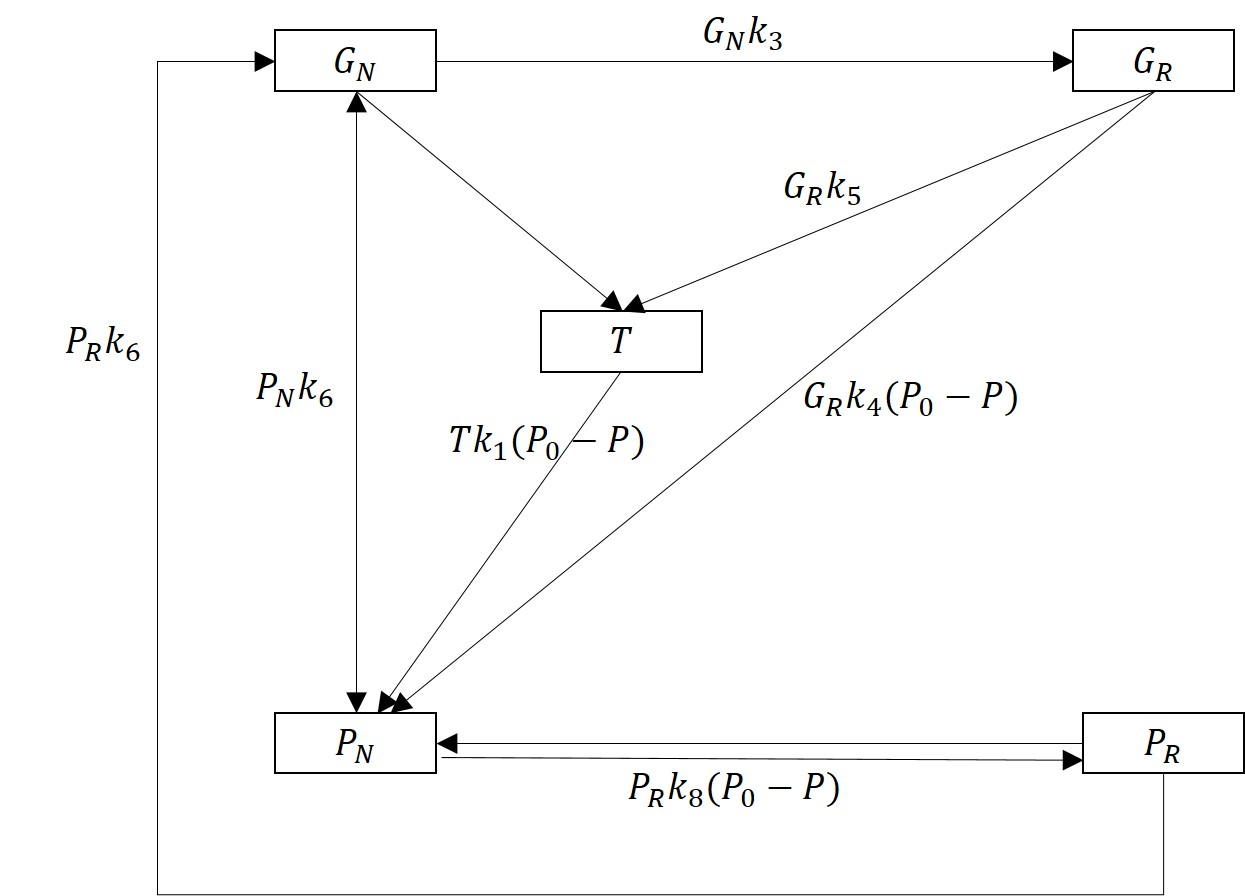
\includegraphics[width=0.9\linewidth]{Report_images/homeless_rates}
	 	
	 	\caption{A diagram to show  flows and and associated rates of households moving  between population groups}
	 	\label{fig:homelessrates}
	 \end{figure}
	 
	These equations implicitly assume that:  
	\begin{itemize}
		\item Birth and death rates can be neglected
		\item No migration in and out of the borough 
		\item Rates depend only on the present circumstances there is no delay e.g. due to administrative processes 
	\end{itemize}

These equations look intractable but substituting $ G_0=P+T+G_r+G_N $ and $ G_0=G+P+T$ reduces the system to 3 differential equations:

\begin{eqnarray}
\frac{dT}{dt}=k_5 G -k_1(P_0 -P)T\\
\frac{dG_R}{dt}=-k_5 G_R+k_3(G_0-P-T-G_R)-k_4(P_0-P)G_R\\
\frac{dP}{dt}=-k_6P+(P_0-P)(k_4G_R+k_1T)
\end{eqnarray}
	
	They looked for equilibrium solutions, setting the time derivatives to zero. They were able to see that a feasible equilibrium solution always exists, where the number of occupied council houses is positive but no greater than the number actually available. 
	
	Looking for analytic solutions of the equations in full generality was deemed unproductive for the short intensive time available in a Study group so focus was moved to looking for numerical solutions. 
	
	Initial values were chosen to represent a typical metropolitan borough. calculations were carried out with numbers of people rather than families. They found that the steady state solution was locally stable but that the values showed high sensitivity from the initial data and values. Thus generalised discussion about results for the ``typical" borough or for all boroughs is not possible. They did however manage to make some useful inferences: 
	

	\begin{itemize}
		\item The populations only settle down to the steady state values over a period of about 30 years. This is a much larger time frame than changes in local and national policies and is large enough that births, deaths and migration should be taken into account. Future work should either aim to increase the complexity of the model to take this into account or should look closer at the initial dynamics and variation. 
		\item Reducing the constant $ k_1 $ by a factor of 10, signifying a change in policy so that much less priority is giving to the homeless on council waiting lists causes very little change apart from a 10-fold increase in the numbers of homeless in the borough. The amount of vacant council property increased a little but not sufficiently to cope with the increase in homeless families. The factor $ k_1 $ is important. 
	\end{itemize}
	
	The work was continued after the study group, including a paper produced based mainly on the work done during the study group \cite{Byatt-Smith2003}. The work was also continued as the MSc project and then the PhD project of Andrew Waugh, supervised by one of the study group attendees Andrew Lacey, at Herriot Watt University. 
	
	We look at one of the extensions he made to the Study Group Model in the form of a points based model \cite{Waugh1999}. This aims to model the mechanisms used to allocate houses to those on the waiting list.  In this model people are either assigned a category or a point score. Categories include:  top medical priority, overcrowding priority or local move priority.   Point scores increase depending on length of time on the waiting list, current situation and homeless status. Suitable houses are primarily offered to those households with a category status, if the house is not suitable or the offer is rejected the offer can be passes to another household in categories or passed down the points. 
	
	An explanation of how these dynamics were implemented is beyond the scope of this case study but in studying the steady state solutions it was found that by removing the priority to the homeless, seen as an extra point allocation, saw an increase in homeless households between 5 and 7 fold and that other populations changed very little, although there was a drop in the number of private sector families satisfactorily housed. Quantitatively, this is the same as the study group model with a much larger rise in homeless households as the result of the policy change. 
	
	Although the model does not include the effects of births, deaths and migration results of policy decisions 40 years in the future are able to be predicted and with some reliability between different models. It demonstrates the scope for this sort of mathematical modelling to have a role in decision making and to be a force for economic and social good. 
	
	\subsection{Case Study 3: Optimisation of the “118” Emergency Management System in Milan \label{Milan} }
	The book ``European Success Stories in Industrial Mathematics" \cite{European2011} contains a wealth of great examples of effective knowledge transfer and collaboration. One particular example, ``Optimisation of the ``118" Emergency Management System in Milan" attracted me because of its real-world importance and its simplicity as a mathematical optimisation problem but also because of a particular sentence: 
	
	\begin{quote}
		``In spite of being developed by academic personnel, the outcome of the project has been actually implemented''
	\end{quote}

	Perhaps, not a sentence I should have taken out of context, but perhaps a typical  opinion of a sceptical academic or company of industrial mathematics and one that needs to be repeatedly challenged.
	

	I follow the 2013 paper by R. Arinhieri, G. Carello and D. Morale \cite{Carello2013}  to describe some fo the work behind this case study.	They focused on 3 areas: evaluation of the current EMS system; study of operational policies which can improve the system performance through a simulation model and using optimisation to fund an alternative set of ambulance posts. 
	\begin{figure}
		\centering
		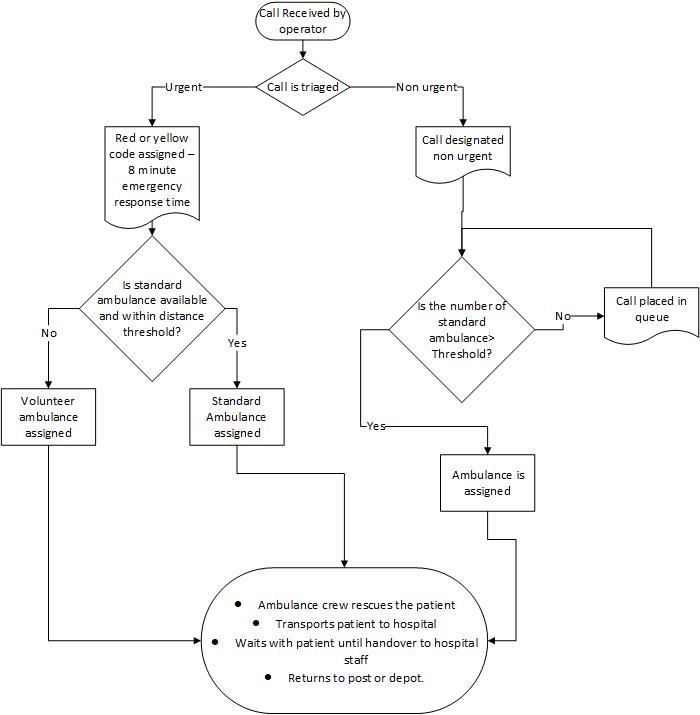
\includegraphics[width=\linewidth]{Report_images/MilanEMS}
		\caption{The process of responding to an emergency call}
		\label{fig:milanems}
	\end{figure}
\paragraph{Evaluation of the current EMS system }
	Figure \ref{fig:milanems} documents  the process of responding to an emergency call. A few points to highlight: 
	\begin{itemize}
		\item Italian law states that urgent calls have to be responded to in 8 minutes in urban areas. This threshold is also a major measure of performance 
		\item The Milano EMS used two types of ambulance: 
		\begin{itemize}
			\item Standard/prepaid ambulances - a set composed of 29 ambulances that are always available. They represent a fixed cost regardless of the number of missions performed. Ambulances are located at ambulance posts ready to be deployed.
			\item ``Volunteer" ambulances - run by various volunteer organisations who own them. They can be summoned if needed and the cost is per mission. They are based at their organisation's headquarters.
		\end{itemize}
		The focus of the work was on the first set: to try and serve the majority of the requests with standard ambulances in order to reduce costs and ensure consistency of quality of care. 
		\item After the ambulance has been assigned to the point were it returns to its post or depot after completing a mission the ambulance is unavailable and cannot be diverted. 
	\end{itemize}
\paragraph{Development of a simulation model in order to test operational policies }
Analysis of the historical data found that there was room for improvement - on average 60.1\% of the urgent calls meet the 8 minute response time with a 95\% confidence interval of $ [56.13\%, 64.06\%] $. Any investment in infrastructure to try and improve these figures would be expensive and with no guarantee of success: a mathematical model could help test different scenarios. 

In the model, ambulance locations are plotted on a map of Milan at each point in time, the speed assigned to each ambulance is a function of the time of the day and the area in which the ambulance is currently located. This is more  computationally intensive compared to an event based model where the movement of an ambulance from a place to another one is usually represented by an new event, the actual movement of the ambulance is not a part of simulation model but this proved to be very fruitful.The model focused on just the set of standard ambulances.

Each emergency request was generated by using real data of a given day, a variety of days were selected to test the model, including some selected critical days which could be representative of emergency scenarios. The model was initialised to model current procedure and for the 7 days worth of events used, the model predicted a that 63.92\% of the urgent calls would be responded to within the 8 minute deadline. This is within the 95\% confidence interval produced from historical data and suggests the simulation is representative of actual EMS behaviour. 

Various parameters could now be varied in order to test different improvement strategies:
\begin{itemize}
	\item \textbf{Increases to  ambulance average speed}: Road improvements, reserved lanes and systems to wave ambulances through traffic lights could all increase average ambulance speed. An average increase of 5km/h was shown in the model to increase the number of urgent calls reached within 8 minutes by approximately 20\%.
	\item \textbf{Adding a new ambulance}:  Adding a new standard ambulance to the fleet would be an expensive investment and the model showed that with the current set of ambulance posts that there would be little improvement in response rates, due to ambulances gathering in a few posts and leading to unbalanced global coverage. 
	\item \textbf{Moving to ``smart" ambulances}: The possibility of summoning an ambulance before it reaches its post on return from a mission, or in redirecting an ambulance on its way to a less urgent mission can be evaluated using the model, because of the agent based approach to modelling ambulances. At the time of the work, ambulances were not equipped with GPS systems and therefore this sort of assignment was not possible. On the heaviest days the model was predicting up to a 20\% improvement in the number of urgent calls responded to within the 8 minute deadline, similar figures to that of increases in ambulance speed but at potentially a much reduced cost and less dependent on external factors such as weather. 
\end{itemize}

\paragraph{Finding an alternative set of ambulance posts}


Low Priority Calls Coverage (LPCC) optimisation model was developed by the authors to take a potential set of posts and solve a minimisation problem, to discover the theoretical minimum number of required ambulances and where their posts should be located. First some definitions of variables:
\begin{itemize}
	\item $V=$ the set of points to be covered. For each point $ i \in V $, $d_i^h$ denotes the amount of high priority demands and $d_i^l$ low priority demands 
	\item $ W= $ the set of candidate post locations. The capacity associated to each post is denoted by $ k_j $.
	\item Let $ W_i^h $ be the set of candidate posts from which a demand point $ i $ can be reached within the 8 minute threshold. 
	We introduce a second time limit in which a certain percentage of non urgent calls must be seen, and similarly let $ W_i^l $ be the set of posts from which $ i $ can be reached in this longer time frame
	\item Let $ y_{ij} $ be the fraction of emergency demand of point $ i  $ served by an ambulance at post $ j $. Similarly $ w_{ij} $ to be the fraction of non urgent demand at point $ i  $ served by an ambulance at point $ j $.
	\item An integer variable $ x_j $ is defined for each post $ j $, representing the number of ambulances assigned to the post, this can be zero.
\end{itemize}

\begin{eqnarray}
\min \ z=\sum_{j\in W} x_j \label{1a}\\
s.t.\ &\sum_{j\in W_i^h} x_j\geq1\ \ &\forall i \in V\label{1b}\\
&\sum_{j\in W_i^h} y_{ij}=1\ \ &\forall i \in V\label{1c}\\
&\sum_{j\in W}w_{ij}=1 \ \ & \forall i\in V \label{1d}\\
&\sum_{i \in V} \sum_{j \in W_i^l} d_i^l w_{ij} \geq q \sum_{i \in V} d_i^l\label{1e}\\
&\sum_{i \in V} (d_i^h y_{ij} +d_i^l w_{ij}) \leq k_jx_j & \forall j \in W\label{1f}\\
&x_j\in Z_+, \ w_{ij} \in [0,1], \ &\forall i \in V,\  \forall j \in W \label{1g}
\end{eqnarray}
Where Eq \ref{1a} is the objective function: to minimise the number of required ambulances. Eq \ref{1b} ensures that there is coverage over all the city. Eq \ref{1c} ensures that urgent calls are served within the given time limit. Eq \ref{1d} guarantees that all the low priority calls can be served by and ambulance at any posts. Eq \ref{1e} forces that a given percentage of the non-urgent calls ate served with a second time limit. Eq \ref{1f} limits the number of missions in a given time frames. Finally \ref{1g} defines the domains of the variables 
 
 
For the solution of Milan the city was divided into 493 grid squares, chosen such that the area in each gird is covered by the same set of candidate post locations. Thus as long as each sub area is covered, all possible areas will also be covered. They set $ V=W $, $ q=0.5 $ and the non-urgent time frame to be 30 minutes. Diagrams showing the grid, the demand for high and low priority calls and the current ambulance positions are shown in figure \ref{fig:ems-milan} . This gives an optimal solution of 25 ambulances.

\begin{figure}
	\centering
	\includegraphics[width=0.9\linewidth]{"Report_images/ems milan"}
	\caption{The 493 grid squares covering the city of Milan, coloured based on demand for ambulances and with current ambulance stations marked on. Diagrams taken from paper \cite{Carello2013}}
	\label{fig:ems-milan}
\end{figure}

The remaining 4 ambulances are then allocated using an iterative procedure where the model from the previous section is used, and ambulance posts given  a ranking determining their utilisation. New posts are added in such a way as to decrease the highest utilisation value , this is iterated until there is a post located for each ambulance. This could also be used to design a set of posts to reach a threshold level of performance.

To conclude, they developed a working simulation of ambulances and calls in the city which they could test policy changes on. They also developed an optimisation problem which could give the minimum number of ambulances required and optimum location of ambulance posts. Combining the two they could recommend locations for any extra ambulances.



	\subsection{Case Study 4: Mathematical Modelling of the Dynamics of Meningococcal Meningitis in Africa \label{Africa }}
The book ``UK Success stories in Industrial Mathematics" \cite{Aston2016} is a collection of cases studies selected from those Impact Case Studies submitted to the 2014 Research Excellence Framework. They are seen as shining examples of the mathematical sciences community engaging with problems and organisations outside of academia. 36 problems were selected out of the 250 submitted for the REF and I aimed to pick just one to write up as a case study- a challenge indeed!


The African meningitis belt spans sub Saharan Africa and see periodic fluctuations of meningococcal meningitis, cases appearing every dry season, drop off over the rainy season and a major epidemic emerges every 6-14 years. Across the world, meningitis causes about 135,000 deaths annually and substantial data is available across the African meningitis belt, so mathematical modelling of epidemiology of meningococcal meningitis could lead to substantial benefits. Indeed, modelling has been attempted by a number of groups but we follow the work by K.B.Blyuss at the University of Sussex described in ``UK Success stories in Industrial Mathematics" and the associated paper \cite{Irving2012}.


\paragraph{Initial Modelling and Identification of Reproduction Number  }
Looking for a simple model the team looked towards the standard SIR model. In the case of meningitis, individuals can be carriers without developing the infection and there is a high ratio of carriers to cases, thus an additional ``carrier" class was a necessary addition, giving 4 classes: 
\begin{itemize}
	\item S= Susceptible
	\item C=Carriers
	\item I=Infected
	\item R=Recovered
\end{itemize}
The total population is $ N=S+C+I+R $. The question of temporary immunity was a major part of this work and they considered a variety of models where there was:
\begin{itemize}
	\item no immunity, and thus no recovered class, recovered individuals went straight  to susceptible 
	\item   immunity only if they have had developed a meningitis infection, if individuals had only been a carrier then they got no immunity
	\item immunity if they had been a carrier, developed the infection or both
\end{itemize}

\begin{figure}
	\centering
	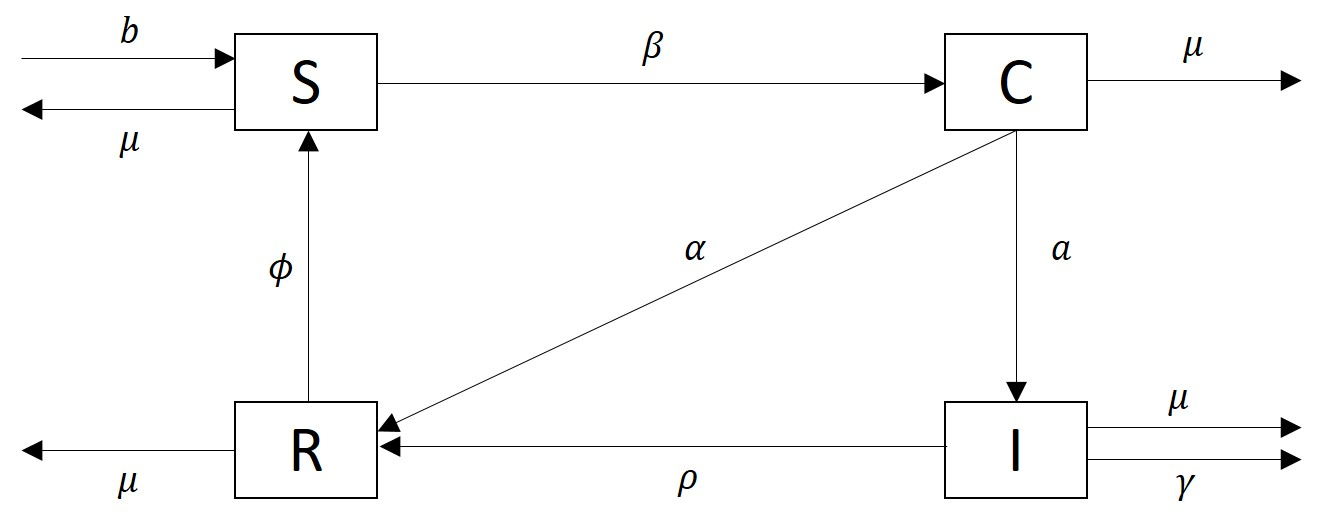
\includegraphics[width=0.9\linewidth]{Report_images/meningitis_model}
	\caption{A diagram to show the flows between population groups in the chosen meningitis model, taken from Fig 2 in paper  \cite{Irving2012}}
	\label{fig:meningitismodel}
\end{figure}



 Modelling all 3 cases they found the best fit to the observed data was the last case and the model shown in Figure \ref{fig:meningitismodel}, with rates defined as followed:
\begin{itemize}
	\item $ \beta =$ the transmission rate
	\item $ a= $ the rate at which carriers develop an invasive disease
	\item $ \alpha =$ the rate at which carriers recover 
	\item $ \rho= $ the rate at which individuals with invasive disease recover
	\item $ \phi = $ the rate at which recovered individuals loose their immunity becoming susceptible again 
	\item $ \mu = $ natural death rate
	\item $ \gamma = $ disease induced death rate

\end{itemize}

The birth rate is chosen to be $ b=\mu N +\gamma I  $ so that the total population $ N=S+C+I+R $ is constant. This assumption is only suitable for relatively short term modelling before the assumptions break down but it is a good starting point and gives equations: 

\begin{eqnarray}
	\frac{dS}{dt}= b +\phi R-\beta \frac{S(C+I)}{N}-\mu S\\
	\frac{dC}{dt}=\beta \frac{S(C+I)}{N}-(a+\alpha+\mu)C\\
	\frac{dI}{dt}=aC-(\rho +\gamma+\mu)I\\
	\frac{dR}{dt}=\rho I +\alpha C-(\phi+\mu)R
\end{eqnarray}
	
	Which under rescaling by $ N $ and using  $ I=S+C+I+R $ to remove $ S $ from the equations gives
	\begin{eqnarray}
	\dot{C}=\beta(1-C-I-R)(C+I)-(a+\alpha+\mu)C\\
	\dot{I}=aC-(\rho+\gamma+\mu)I\\
	\dot{R}=\rho I+\alpha C-(\phi+\mu)R
	\end{eqnarray}
	
	We look for steady state solutions when $ \dot{C}=\dot{I}=\dot{R}=0 $. Messy calculations but one finds:
	\begin{eqnarray}
	C^*=\lambda (\phi+\mu)(\rho+\gamma+\mu)\\
	I^*=\lambda a(\phi+\mu)\\
	R^*=\lambda(\alpha(\rho+\gamma+\mu)+\rho\alpha)
	\end{eqnarray}
	
	Where $ \lambda $ is a proportionality constant that can be found by subbing into $  \dot{C}=0 $ giving $ \lambda=0 $ or:
	
	\begin{eqnarray}
	\lambda=\frac{\beta(\gamma+\rho+\mu+a)-(\gamma+\rho+\mu)(\alpha+a+\mu)}{\beta(\rho+\mu+a)[(\rho+\gamma+\mu)(\phi+\mu+\alpha)+a(\phi+\mu+\rho)]}\\
	=\frac{(\rho+\gamma+\mu)(a+\alpha+\mu)}{\beta(\rho+\mu+a)[(\rho+\gamma+\mu)(\phi+\mu+\alpha)+a(\phi+\mu+\rho)]}\frac{\beta(\gamma+\rho+\mu+a)-(\gamma+\rho+\mu)(\alpha+a+\mu)}{(\rho+\gamma+\mu)(a+\alpha+\mu)}\\
	=\frac{(\rho+\gamma+\mu)(a+\alpha+\mu)}{\beta(\rho+\mu+a)[(\rho+\gamma+\mu)(\phi+\mu+\alpha)+a(\phi+\mu+\rho)]}\left( \frac{\beta(\gamma+\rho+\mu+a)}{(\rho+\gamma+\mu)(a+\alpha+\mu)}-1\right) 
	\end{eqnarray}
	
	
	An important quantity to identify when looking at epidemiology models is the reproduction number,  $  R_0 $. As defined in \cite{VanDenDriessche} it is such that if $ R_0 < 1 $, then the disease free  steady state $ (C,I,R)=(0,0,0) $ is stable, and the disease cannot invade the population, but if $  R_0 > 1 $, the disease free steady-state is unstable and an epidemic can take hold. 
	For $ R_0>1 $ a new stable stationary point should exist for values of $ C,I,R>0 $.
	In our case looking at our two potential steady states and the equations for $\lambda$ we find that in order for $C^*, I^*, R^*>0$ we require: 
	
	\begin{eqnarray}
	R_0=\frac{\beta(\gamma+\rho+\mu+a)}{(\gamma+\rho+\mu)(a+\alpha+\mu )}>1
	\end{eqnarray}
	Giving us the reproduction number and valuable information about in which circumstances meningitis will spread or be contained. 
	
Again using \cite{VanDenDriessche}  a more qualitative description for the reproduction number is  the number of new infections produced by a typical infective individual in a population at a disease free steady state.  If $ R_0 < 1 $, then on average an infected individual produces less than one new infected	individual over the course of its infectious period, and the infection cannot grow. Conversely, if 	$ R_0 > 1 $, then each infected individual produces, on average, more than one new infection, and the disease can invade the population. 


We consider adding a new carrier to an otherwise healthy population. Two things can happen, the carrier can directly infect healthy members of the population or the carrier can become infected and then infect healthy members of the population. 

The expected amount of time the carrier remains a carrier is
 \begin{eqnarray}
\frac{1}{a+\alpha+\mu}
\end{eqnarray}
and as a carrier they infect members of the general population at rate $ \beta $ giving expected number of people infected by a single carrier that doesn't become infected is:
 \begin{eqnarray}
\frac{\beta}{a+\alpha+\mu}
\end{eqnarray}

The carrier becomes infected with probability 
 \begin{eqnarray}
\frac{a}{a+\alpha+\mu}
\end{eqnarray}
calculated from the expected time the carrier remains a carrier multiplied by the rate of contracting the infection. The expected time they remain infected is: 
 \begin{eqnarray}
\frac{1}{\rho+\delta+\mu }
\end{eqnarray}
and they infect healthy individuals with rate $\beta  $

Thus the expected number of new cases is: 

\begin{eqnarray}
R_0=\frac{\beta}{a+\alpha+\mu}+\frac{a}{a+\alpha+\mu}\frac{\beta}{\rho+\delta+\mu }\\
=\frac{\beta(\gamma+\rho+\mu+a)}{(\gamma+\rho+\mu)(a+\alpha+\mu )}
\end{eqnarray}
Matching the result from before.

\paragraph{Adding the seasonal effects  }


To try and explain the seasonal variations in the number of cases, they introduced a seasonally varying rate of disease transmission:
\begin{eqnarray}
\beta(t)=\beta_0(1+\epsilon_\beta \cos(2\pi t))
\end{eqnarray}
	
The model then exhibits a wide variety of dynamical behaviours and importantly, sees chaotic behaviour for a range of values of $\phi$ which is significant as $\frac{1}{\phi}$ is the expected duration of temporary immunity. Simulations suggest that that the model is able to produce the regular annual epidemics as well as epidemics with larger periods, can produce different amplitudes of epidemics and chaotic behaviour such as which is seen in the data. The longer inter epidemic periods, such as the 6-14years seen in the data corresponds to $\frac{1}{\phi}\approx 2 $ years.  
\paragraph{Impact}

\begin{itemize}
	\item The model highlighted the important role of the temporary immunity and the value of the constant $\phi$. A focus on computing an accurate value for this constant or working clinically to alter its value could be hugely beneficial
	\item An accurate value of the reproduction rate, $ R_0 $ is important when optimising vaccination deployment, reducing costs and increasing effectiveness. 
	\item Future work could look at including spatial effects, potentially including satellite and meteorological data. An advance disease warning system, for the larger deadlier outbreaks every 6-14 years would be hugely beneficial. 
\end{itemize}
	\pagebreak
	\section{Extended Case Study - High Intensity Focused Ultrasound \label{extended}}
	
	High Intensity Focused Ultrasound (HIFU) is a non-invasive technique to enhance biological therapies by exposing tissues to acoustic energy. Applications include:
	\begin{itemize}
		\item Destroying cancerous tissue using thermal hyperthermia 
		\item Localised drug delivery 
		\item Functional/structural modification of tissues
	\end{itemize}
In addition paediatric foetal application are beginning to be explored due to the potential to deliver a non-ionizing energy based therapy, in a non-invasive manner. 

The technique can be described very basically as: 
	\begin{itemize}
		\item A transducer produces an ultrasound signal focused on a region, $8 mm\times2 mm\times2 mm$
		\item Pressure variations due to the ultrasound lead to a temperature source $Q(\textbf{x},t)$ in the region
		\item Temperature $T(\textbf{x},t)$ changes due to the action of the source, diffusion and perfusion due to blood flow. 
		\item High temperatures over a sustained time lead to tissue damage. 
	\end{itemize}
	
	The problem of developing this idea into a usable medical technique can be split into three areas: focusing the ultrasound signal onto the region, controlling the temperature levels  and imaging the procedure. 
	
	\subsection{Background}
	\subsubsection{Set Up}
	Clinical adoption of HIFU has expanded rapidly in recent years partly due to better visualisation and thermometry tools. A typical set up is shown in Figure \ref{fig:howitworks}
			\begin{figure}
		\centering
		\begin{center}$
			\begin{array}{c}
			\includegraphics[width=0.9\linewidth]{"Report_images/howitworks"} \\
			\includegraphics[width=0.5\linewidth]{"Report_images/howitworks2"}\\
			\includegraphics[width=0.9\linewidth]{"Report_images/howitworks3"}
			\end{array}$
		\end{center}
		
		\caption{The set-up of MRI with integrated HIFU, taken from material used during  the study group }
		\label{fig:howitworks}
	\end{figure}
	\subsubsection{Imaging}
	Safety and efficacy of the treatment requires accurate temperature measurement throughout the thermal procedure of the target tissue but also of surrounding structures.
	
	The method has shown some success in uterine fibroids, prostate cancer and liver tumours but application of the method for treatment of brain tissue remains a challenge due to strong aberration due to the skull bone, defocuses the beam and results in a loss of acoustic pressure. Thus another important use of imagery to detect the location of the beam and then to correct for the defocusing to refocus the beam. 
	
	MRI thermometry, is a method where a traditional MRI scanner can be used to measure temperature. Temperature measurement is based on the water proton resonance frequency (PRF) shift induced phased differences between dynamic frames. From MR dynamic phase images a relative frequency shift is calculated:
	
	\begin{equation}
	\Delta T= \frac{\Delta \phi}{2 \pi \alpha \gamma B_0 T_E}
	\end{equation}
	
	Where: 
	\begin{itemize}
		\item $\Delta \Phi $ = phase shift 
		\item $\alpha$ = Temperature sensitivity coefficient 
		\item $\gamma$ = gyromagnetic ratio
		\item $B_0$ = magnetic field strength
		\item $T_E$ = echo time 
	\end{itemize}

	Temperature maps are calculated in real time and displayed as overlays on the magnitude image. An example can be seen in Figure \ref{fig:mriimage}.
	
	\begin{figure}
		\centering
		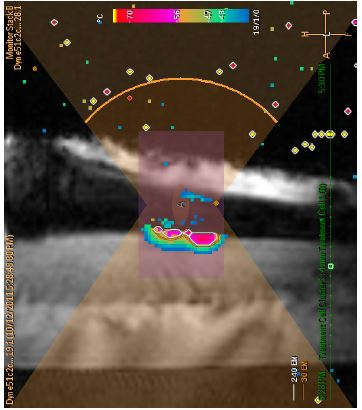
\includegraphics[width=0.7\linewidth]{Report_images/MRIimage}
		\caption{Temperature maps are calculated in real time and displayed as overlays on the magnitude image}
		\label{fig:mriimage}
	\end{figure}
	
	The Review Paper by Viola Reike and Kim Butts Pauly on MR thermometry \cite{Rieke2008} gives a good overview of the science as well as some of the drawbacks.  	It discusses how the target for many ablation procedures lies in the abdomen where normal body motions such as breathing have a significant effect and that more reliable and robust motion insensitive acquisition and reconstruction techniques need to be developed.
	 
	Other drawbacks to MR thermometry is that temperature in bone and fat tissue cannot be measured with the PRF method and the phase of a MR image is sensitive to disturbances such as transducer movement and magnetic field drift. As noted in paper \cite{Hosseini2018} there are also high computational costs. Finally, as highlighted in the initial study group proposal that MR thermometry does not provide high spatial resolution so partial volume effects, where the averaging of temperature across a size of a voxel when the voxel contains heterogeneous tissues, causes temperature to be underestimated.
	
	

	
	\subsubsection{Focusing the ultrasound signal}
	
	When considering the focusing of the ultrasound signal there are many different methods being investigated. Not the main focus of this report but I couldn't resist looking at two possible avenues of investigation : 
	\begin{itemize}
		\item  \textit{Magnetic Resonance acoustic radiation force imaging} (MR-ARFI) is described in a paper by Bambad Hosseini et al	\cite{Hosseini2018}. Here the aim is to obtain measurements of the intensity of the acoustic field at the focal point. MR-ARFI uses low-duty cycle HIFU pulses that cause tissue displacement in the order of microns at the focal point of the beam. These can then be measured with the MRI using gradient pulses and displacement maps are generated that can be used to verify and correct the degree of focusing of the HIFU beam. The main drawback of this technique is the number of sonication tests required which leads to a long acquisition time for the MRI data. The paper suggests that this number of sonication tests can be reduced by casting the problem within the framework of Bayesian Inverse Problems allowing for a stable estimations of the aberrations with very noisy data and few sonication tests. The benefits of using a Bayesian model is also that associated uncertainties in the estimate are also given.
		\item \textit{Time Reversal Acoustics} is described in a very accessible article for Scientific American by Matthias Fink, \cite{Fink1999}. Put very simply, an acoustic time reversal mirror operates in two steps. In the first step a source inside the area of interest emits sound waves that propagate out. They are distorted by inhomogeneities in the medium. These are then detected by a set of transducers in an array surrounding the region of interest and the signals are fed to a computer. In the second step, the signal is time reversed and the transducers play back the signal. The original wave is recreated, but travelling backwards, retracing its steps through the medium and refocusing on the original source.  The two steps are shown in diagrams in Figure \ref{fig:time-reversal-cavity}. 
		
		The time symmetry  and linearity of the wave equation means that the return wave is physically possible, it satisfies all the correct equations. The linear constructive and destructive interference properties of waves also mean that small errors and noise do not grow exponentially, but instead remain linear and result in only minor defocusing around the original source.
		\begin{figure}
			\centering
			\includegraphics[width=\linewidth]{"Report_images/Time-reversal cavity"}
			\caption{A diagram to show the two steps of the time reversal process. The image is taken from previous work by this author \cite{Duff2018} and is inspired by figure 4 in paper \cite{Fink1992}.} 
			\label{fig:time-reversal-cavity}
		\end{figure}
		
		A very interesting phenomena, is that when the array of transducers is relatively small, and a distance away from the source, inhomogeneities in the media actually improve the focusing, the opposite of what is to be expected. See for example paper \cite{Borcea2002} for further details. 
		
		A major application is that of lithotripsy, the breaking up of kidney stones, here there is no obvious source of sound waves. Instead one part of the array sends a brief pulse out into the media (the body) and that wave is reflected back to the array by reflectors in the media. This is recorded time reversed and remitted, focusing back on the reflectors. If there are several targets in the media, repeating of this process eventually focuses on the brightest reflector. 
	The task of locating kidney stones in real time where there is movement due to breathing and the destruction process is very difficult by conventional methods such as x-rays. After several iterations of the pulse-echo time reversal process the  waves focus on the most reflective area of the stone. Intermittent amplified pulses can then be used to shatter the stone. 
		
		Applications to thermal hyperthermia have been investigated. Fink's group have looked at focusing ultrasound waves through the skull using a modified play back algorithm to correct for the strong absorbing properties of the skull breaking the time reversal symmetry. They were successfully able to focus on a 1.5 mm spot. 
		
		A paper by Cochard et al from 2009 \cite{Cochard2009}, uses a method that decomposes the time reversal operator, the DORT method, to assist focusing through the ribs. The DORT method very roughly finds that the singular values of the time reversal operator  which correspond to the reflectors in the media. The brightest reflectors, with highest singular values are that of the ribs. Finding the corresponding vectors in the singular value decomposition finds those vectors that will focus on the ribs. An excitation vector orthogonal to the subspace of emissions focusing on the ribs applied to the transducers should avoid focusing on the ribs and allow treatment of organs inside the rib cage. 
		
	
	\end{itemize}
	
		
		
	
	\subsubsection{Modelling Heat transfer and thermal dose}
	

	Proposed in the 1940s, the Pennes Bioheat Transfer Model, \cite{Pennes1948} models heat transfer in the body due to externally applied heating/cooling sources. It has three terms, a diffusion term, an external heating term, and a convection term due to the perfusion of heat due to blood flow. The model accounts for the thermal conductivity, specific heat capacity and blood perfusion of specific tissue types. 
	\begin{equation}
		\boxed{\rho c \frac{\partial T}{\partial t}= \nabla\cdot k \nabla T-\omega c_b (T-T_b)+Q}
	\end{equation}
	where:
	
	\begin{itemize}
		\item $ \rho = $ Tissue density[$ kg/m^3 $]
		\item  $ c= $ Specific heat capacity [$ J/kg/\degree C  $]
		\item $ k= $ Thermal conductivity  [$ W/m/\degree C $]
		\item $ \omega = $ Blood perfusion [$ kg/m^3/s $]
		\item $ Q= $ Heat deposition from ultrasound $ [W/m^3 $]
		\item $ T_b= $ Arterial blood temperature [$ 37\degree C $]
		\item $ t= $ Time [$ s $]
	\end{itemize}
	
	
	
	\begin{figure}
		\centering
		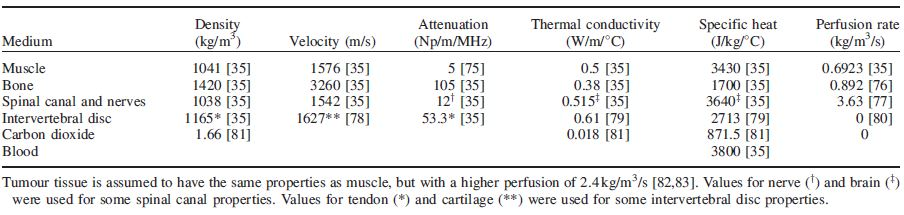
\includegraphics[width=1\linewidth]{Report_images/tissueproperties}
		\caption{Material properties of tissues, taken from paper \cite{Scott2014}.}
		\label{fig:tissueproperties}
	\end{figure}
	
	Initially, Harry Pennes experimented on patients by inserting thermocouples into patients' forearms but the model has been validated over the years against other models and is applicable to many different heating sources and types. Values for specific tissue types are available and are shown in Figure \ref{fig:tissueproperties}. 
	
	However, there is not one specific temperature at which all cells automatically ablate, the effects are cumulative and vary between types of tissue. Different temperatures during heating and cooling, diffusion from the target area and possible patient movement all contribute to uneven heating in different areas. Therefore, some sort of normalisation is required to calculate the effect on each individual cell in the form thermal dose measure  from which effective dose and dangerous levels can be estimated. 
	
	
	
	The most commonly used model, \cite{Sapareto1984a},  measures thermal dose as a time integral calculated over the treatment length:
	
\begin{equation}
\boxed{TD(t)=\int_{0}^{t}r^{43-T(t)}dt,\ \ \text{where  } r=
\begin{cases}
0.25, & \text{if}\ T\leq 43 \degree C \\
0.5, & \text{if}\ T>43 \degree C 
\end{cases}}
\label{Sapereto}
\end{equation}
	
	The value taken as sufficient ``dose" to cause thermal necrosis in soft tissue is 240 EM (equivalent minutes) at $43 \degree C $. One can also calculate that it takes just a 1 second exposure at $57 \degree C $ to give a thermal dose of 273 EM and thermal necrosis. For every degree above  $43 \degree C $ the required time to coagulate the tissue halves. 
	
	The model has its advantages for HIFU: importantly it is valid for the high temperatures seen in HIFU and it is valid for tissues with different thermal sensitivity although the threshold for thermal dose required for cell death changes. 
	
	Showing this model to mathematicians with no knowledge of biology but skills in modelling, their first questions are where does $ r $ come from and what is special about $43 \degree C $? The model is not very intuitive. From a more practical point of view, the model has its draw backs as there is a non linear response between temperature and cell death - higher probability of dying with increasing temperature and time exposure. Also, measuring dose does not directly predict damage, for example: you can't say that if you give an area a thermal dose of 120EM then approximately half the cells will have been damaged. Finally, tissues have varying thermal sensitivity and will ablate at different thermal doses which will add extra complexity to the model.
	
		An alternative model for cell damage was introduced in  paper  \cite{Zhou2007}. Zhou et al suggest that damage is the result of a chemical reaction:
		\begin{equation}
		P\rightarrow D
		\end{equation}
		
		Where P represents a healthy folded protein and D a denatured protein. The irreversible process of protein denaturization occurs at an Arrhenuius reaction rate:
		
		\begin{equation}
			\boxed{r(T)=A\exp\left( \frac{E}{RT}\right) }.
		\end{equation}	
		Where A is a frequency factor, E the energy of activation of the denaturization reaction, R is the universal gas constant and T is the absolute temperature of the tissue. From this a damage fraction can be calculated:
		\begin{equation}
			\boxed{\Omega(t)=\log\left( \frac{P_0}{P(t)}\right) =\int_{0}^{t}A\exp\left( \frac{E}{RT}\right) dt}
		\end{equation}
		where $ P_0$ is the initial amount of folded protein.
		
		The idea is that a value $\Omega_\theta$, a damage threshold, is found such that $\Omega>\Omega_\theta$ then irreparable damage has occurred. In the study group a value $\Omega_\theta=0.63$ is chosen for muscle. 
		
		
	 	The parameters, A, E and $\Omega_\theta$, the damage threshold, can be varied to match different tissue types. Originally developed for use to model damage from a laser so perhaps more experimental work needed to verify this for lower temperatures. However, this model is intuitive and easy to implement numerically by writing the integral as a sum and updating the damage fraction with each iteration. 
	 	
	 	
	 	\subsubsection{Study group work}
	 	The problem challenges for the study group were: 
	 	\begin{enumerate}
	 		\item Can a tissue type dependant thermal dose model (similar to the Pennes Bioheat model for tissue heating) be derived that takes into account the thermal conductivity, thermal diffusion, specific heat, and perfusion of the tissue of interest and surrounding structures?
	 	\item 	Can a spatially dependant (and perhaps a patient specific) thermal dose model be derived which can work directly with intra-operative temperature measurements to better predict the volume of ablated tissue during a MR-HIFU treatment?
	 	\end{enumerate}
	 	
	 	Due to the short time frame of a study group they decided to focus on a couple of problems: 
	 	
	 	\begin{itemize}
	 		\item Find a semi-analytic expression for the spatially extended
	 	temperature field $ T(x; t) $
	 	\item Obtain numerical computations of a simplified model which
	 	allows us to look at the effects of parameter variation and
	 	compare these with calculations from a more sophisticated
	 	model
	 	\item Determine useful and usable models for the spatial tissue
	 	damage which depend on material parameters which takes
	 	into account the thermal dose, thermal conductivity, thermal
	 	diffusion, specific heat, and perfusion of the issue of interest
	 	and surrounding structures.
	 	\end{itemize}
	 	They focused on looking at muscle tissue where the approximate values are:
	 	\begin{itemize}
	 		\item $\rho c \approx 3 \times 10^6$
	 		\item $\gamma \approx 2000$
	 		\item $Q \approx 4\rho c-10 \rho c$
	 		\item length scale of $L \approx 10^{-3}$
	 		\item $k \approx 1/2$
	 	\end{itemize}
 	
 	Thus looking at the size of terms in the Pennes Bioheat transfer equation:
 	\begin{itemize}
 		\item $\nabla (k\nabla T) \approx 10^6$
 		\item $ \gamma (T-T_b) \approx 10^3$
 		\item $ Q \approx 10^6$
 	\end{itemize}
 and hence it can be concluded that at the focus, perfusion is unimportant unless we are close to a major blood vessel.  $ Q $ diminishes rapidly away from the focus, and so both perfusion and diffusion act together to reduce the temperature. 
 
 They chose to rewrite the Pennes equation as a radially symmetric system close to the focus. The used the approximation: 
 \begin{equation}
 Q=Q_0 \rho c \left(\frac{J_1\left(\frac{r}{L}\right)}{\frac{r}{L}}\right)^2= Q_0\rho c \left(\frac{J_1(s)}{s}\right)^2
 \end{equation}
 where $s=r/L$ and this gives the equation:
 \begin{equation}
 T_t=\frac{1}{6s}(sT)_ss-\frac{2}{3}\times 10^{-3}(T-T_b)+Q_0 \left(\frac{J_1(s)}{s}\right)^2
 \end{equation}
 with initial conditions $$ T_s(0)=0 , \ \ \ T(\infty)=T_b .$$
 
 This can be solved numerically with the Crank Nicholson method, with rapid convergence,  utilising the sparsity of the resulting matrices. 
 
 They ran with $Q_0=5$ for $0<t<30$ and then for $Q_0=0$ for $t>30$. Reproducing this method I get the result shown in Figure   \ref{fig:studygroupcode}. This compared well to the results from more complex 3D models and can be tested by using $ Q=\sin(r)/r $ which would give an analytic solution. It is also exceptionally quick to run and constants can easily be altered for different mediums. 
 
 However, the 1D spherically symmetric model does not give many options for inhomogeneities in the region of interest. For example heating near a bone or near a major blood vessel, a major part of the first question posed for the study group.
 \begin{figure}
 	\centering
 	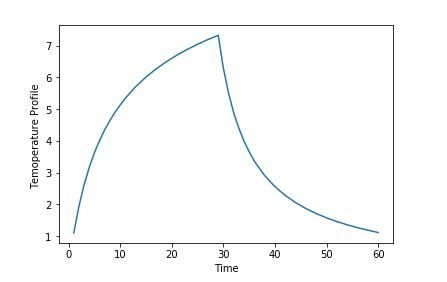
\includegraphics[width=0.7\linewidth]{Report_images/studygroupcode}
 	\caption{A reproduction of the graph produced during the study group of temperature profile against time, where there is heating for the first 30sec before the tissue is left to cool}
 	\label{fig:studygroupcode}
 \end{figure}
\subsection{Current Work } 
 \subsubsection{Aims}   
  Following on from the study group, the aims of my short project are to: 
 \begin{itemize}
 	\item  Work on modelling heat transfer which encompasses: 
 	\begin{itemize}
 		\item  Thermal conductivity
 		\item  Thermal diffusion 
 		\item  Specific heat capacity
 		\item  Perfusion 
 	\end{itemize}
 	of the tissue of interest but also including its surrounding structures primarily bone in our case.
 	
 	\item To use this  to model thermal dose and thermal damage of the tissues and surrounding structures. 
 \end{itemize}

\subsubsection{(Very) Brief literature review}

There are two papers I found interesting reading when considering temperature modelling with more complex structures:
\begin{itemize}
	\item A 2014 paper in the international Journal of Hyperthermia by Scott et al \cite{Scott2014} looks at theoretical parametric and patient specific models to assess the feasibility of ultrasound ablation of tumours in or near the spine. They used the Pennes Bioheat transfer equations, with the properties from table \ref{fig:tissueproperties} and equation \ref{Sapereto} gives the thermal dose. They modelled $ Q $ as an exponential function:
	\begin{equation}
	Q=2\alpha I=2\tau \alpha I_s\frac{r_t}{r}\exp\left( -2\int_{r_t}^r \mu dr' \right) \label{ComplicatedQ}
	\end{equation}
	where $ \alpha $ is the ultrasound absorption coefficient, I is the acoustic intensity, $ \tau $ is the transmission coefficient, $ I_s $ is the acoustic intensity on the transducer surface, $ r_t $ is the transducer radius, r is the radial distance from the transducers central axis and $ \mu $ is the ultrasound attenuation coefficient.
	
	Finite element analysis with mesh sizes ranging from 0.4 mm on inner surfaces to 5 mm overall were used with gradual transitions in mesh size. Dirichlet boundary conditions were used with $ 37\degree C $ on the outermost tissue boundaries and convective boundary conditions applied between inner boundaries between different structures. Patient specific models were generated based on 11 real life patients, and tumours and analysed using COMSOL multiphysics 4.3 in conjunction with MATLAB. 
	
	They found that bone adjacent to or surrounding a tumour can augment heating at the tumour boundaries, shortening treatment times while containing heating to the target volume, as bone has a high ultrasound absorption coefficient and is thermally and acoustically insulation. They were also able to give some estimates of the minimum amount of bone required to protect nerve structures with a maximum thermal dose of  3.6EM to the nerve tissues. They found that in 5 cases of patient models, complete ablation of tumours was modelled as possible and in another 4 cases 94.6\%-100\% of the tumour could be ablated. The model could be very valuable in assessing whether treatment could be viable and planning for treatment. 
	\item Also the 2012 paper by Sassaroli et al for the Scientific World Journal \cite{Sassaroli2012},  look at the potential impact of vasculature on the temperature achieved. They looked at the cases of a homogeneous block of muscle like tissue with either one vessel, a vessel pair or multiple vessel pairs. Like the previous paper they used the Pennes Bioheat transfer equation and equation \ref{Sapereto}. 
	
	For the case of a single vessel  with the flow velocity of the artery running along the axial direction of the transducer, with the ultrasound focus at the blood vessel centre and blood flow opposite to the ultrasound beam propagation. With this geometry the model can be solved using cylindrical symmetry simplifying the calculations.  Results for different sized blood vessels are shown in figure \ref{fig:sassaroli}. They found that temperatures favourable to thermal damage can be reached by that the temperature distribution is highly inhomogeneous due to the blood vessel presence.  Varying the size of blood vessels they found that the largest vessels were very difficult to heat but those less than 0.3 mm in radius heated easily to the nearby tissue temperature.
	\begin{figure}
		\centering
		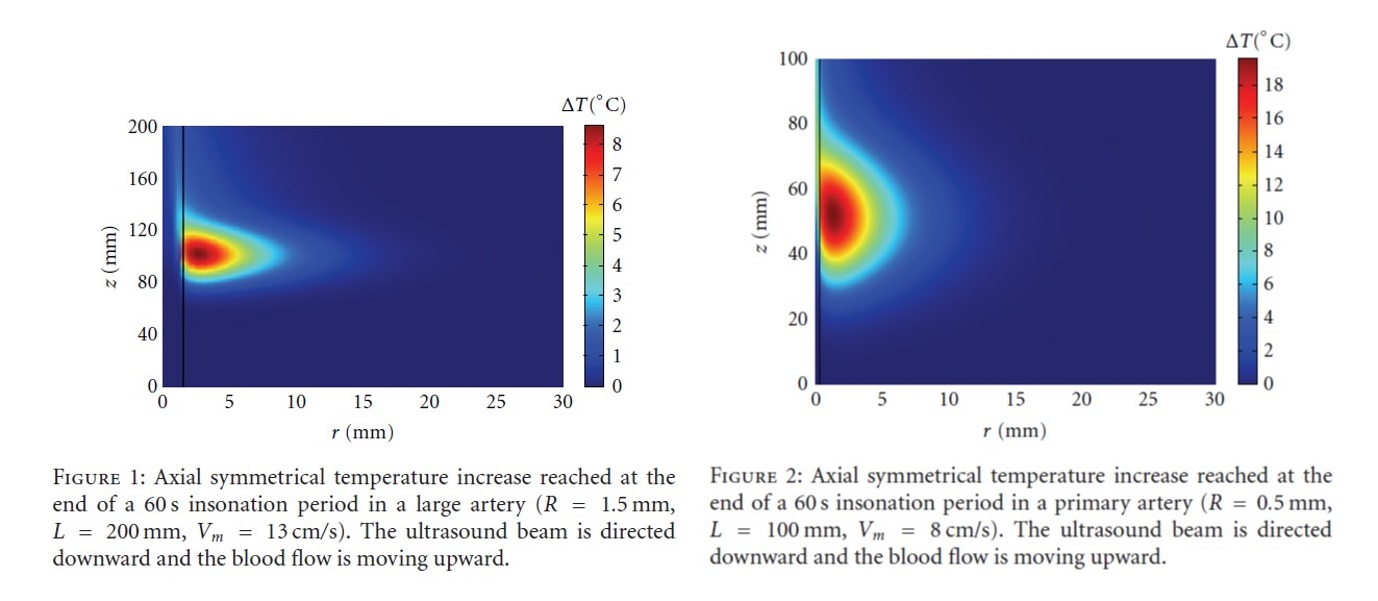
\includegraphics[width=\linewidth]{Report_images/sassaroli}
		\caption{Results of a cylindrically symmetric model of HIFU heating at the centre of different sized blood vessels. Taken from paper \cite{Sassaroli2012}}
		\label{fig:sassaroli}
	\end{figure}
	
	In the cases of multiple blood vessels they were able to solve the full inhomogeneous model using COMSOL and Matlab and were able to investigate how over a treatment period the focus and power of the ultrasound could be varied in order to try and give a uniform thermal dose despite the cooling effects of the blood vessels.   
\end{itemize}





 
 \subsubsection{2D model homogeneous muscle tissue}
Initially, I looked at creating a 2D model of the set up modelled in the study group. Thus thermal conductivity, thermal diffusion, specific heat capacity, perfusion constants are taken for muscle.
$ Q $ was modelled as a Gaussian at the centre of the area of interest and a constant temperature of 37 degrees  were taken as Dirichlet boundary conditions 

To get some feeling for the equations initially I discretised the problem using a central difference in space and a forward difference in time. Thus if $T^i_{m,n}= T(i\delta t, m\delta x, n\delta y)$ we have that:

\begin{eqnarray}
\rho c \left( \frac{T^{i+1}_{m,n}-T^i_{m,n}}{\delta t}\right)= k\left[  \frac{(T^i_{m+1,n}-2T^i_{m,n}+T^i_{m-1,n})}{(\delta x)^2}+\frac{(T^i_{m,n+1}-2T^i_{m,n}+T^i_{m,n-1})}{(\delta y)^2}\right] \\ +Q^i_{m,n}-\omega c_b(T^i_{m,n}-T_b) \nonumber \label{euler method}
\end{eqnarray}

This is an explicit method and so easy to implement and indeed the images produced, shown in figure \ref{fig:forwardcentraldifference}, seem to make sense from what we expect physically. 

\begin{figure}
	\centering
	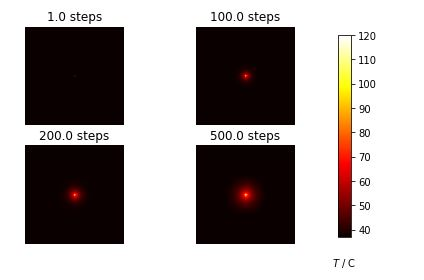
\includegraphics[width=0.9\linewidth]{Report_images/forward_central_difference}
	\caption{Heating modelled using a forward difference in time and central difference in space.}
	\label{fig:forwardcentraldifference}
\end{figure}

Although I am able to make use of some of the numpy linear algebra routines in built into python, making this code relatively quick to run, adding biological structure by changing the values of the constants depending on location in the array means many of these routines cannot be exploited, increasing running cost. We do note however that due to the large values of $\rho c$ then this method should be stable for a range of values of $\delta t$ and $\delta x$.

\begin{figure}
	\centering
	\includegraphics[width=\linewidth]{"Report_images/2d_homogenous heating and cooling"}
	\caption{2D model of heating and cooling of muscle tissue. The first line is heating, second line cooling.}
	\label{fig:2dhomogenous-heating-and-cooling}
\end{figure}
This can be shown by using a  1D version of equation \ref{euler method}:

\begin{eqnarray}
T^{i+1}_m=T^i_m+\frac{k\delta t}{\rho c (\delta x)^2}[T^i_{m-1}-2T^i_m+T^i_{m+1}]+\frac{\delta t}{\rho c}[Q^i_m-\omega c_b (T^i_m-37)]
\end{eqnarray} 

Which can be written in the form $$ T_{\delta x}^{n+1}=A_{\delta x}T_{\delta x}^{n}+f_{\delta x}^{n} $$
where 

$$ A_{\delta x}= \left( \begin{array}{ccccc}
1- 2\frac{k \delta t}{(\delta x)^2 \rho c} -\frac{\delta t \omega c_b}{\rho c }& \frac{k \delta t}{(\delta x)^2 \rho c} & 0 &\cdots  &0  \\ 
\frac{k \delta t}{(\delta x)^2 \rho c}& \ddots  & \ddots  &  & \vdots \\ 
0& \ddots  &  & \ddots  & 0 \\ 
0&  & \ddots  & \ddots  & \frac{k \delta t}{(\delta x)^2 \rho c} \\ 
0& \cdots &  0&\frac{k \delta t}{(\delta x)^2 \rho c}  & 1- 2\frac{k \delta t}{(\delta x)^2 \rho c} -\frac{\delta t \omega c_b}{\rho c }
\end{array}  \right)  $$

This is a  Toeplitz tridiagonal matrix and thus it has eigenvalues:

\begin{eqnarray}
\lambda_k = 1-\frac{\delta t \omega c_b}{\rho c}-4\frac{k \delta t}{(\delta x)^2 \rho c}\sin^2\left( \frac{k\pi}{2d+2}\right) 
\end{eqnarray}

Where $D$ is the matrix dimension and $k=1,...,d$. For stability, as our matrix is symmetric and thus normal, we require that the absolute values of the  eigenvalues are less than one. As the second and third term are both very small due to $\rho c \approx 10^6$, the method  should be stable for a large range of $ \delta t $ and $ \delta x $


\begin{figure}
	\centering
	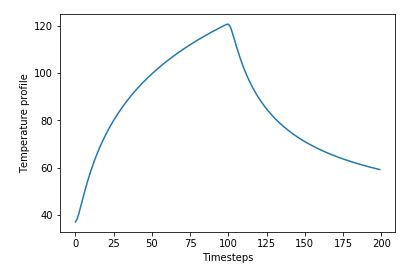
\includegraphics[width=0.7\linewidth]{Report_images/study_group_code_2D_model}
	\caption{Temperature of a point a short distance from the focus measured throughout a heating and cooling period}
	\label{fig:studygroupcode2dmodel}
\end{figure}


To reduce computational cost we tried a semi-discretisation to give an ODE in time, and then used python's inbuilt ODE solver, odeint. This is based on the  lsoda from the FORTRAN library odepack which automatically selects between non-stiff (Adams) and stiff (BDF) methods. The ODE is given by:

\begin{eqnarray}
\rho c \frac{dT}{dt}= k\left[  \frac{(T^i_{m+1,n}-2T^i_{m,n}+T^i_{m-1,n})}{(\delta x)^2}+\frac{(T^i_{m,n+1}-2T^i_{m,n}+T^i_{m,n-1})}{(\delta y)^2}\right] +Q^i_{m,n}-\omega c_b(T^i_{m,n}-T_b).
\end{eqnarray}

Ignoring the perfusion term, valid because it is small, we can get models for heating and cooling as given in \ref{fig:2dhomogenous-heating-and-cooling}, again there is nothing unexpected. Additionally, recording temperatures from a small distance away from the focus and plotting a graph of temperature against time gives the result as shown in figure \ref{fig:studygroupcode2dmodel}. This is similar to the temperature profile shown in figure \ref{fig:studygroupcode}. For the moment we ignore exact units, although we note that the temperature values produced seem realistic. 

Adding back in the perfusion term, despite how small it is, has a dramatic effect on the numerical stability. Problems originating at the boundary are particularly common. Examples are shown in figure \ref{fig:instability}.



\begin{figure}
	\centering
	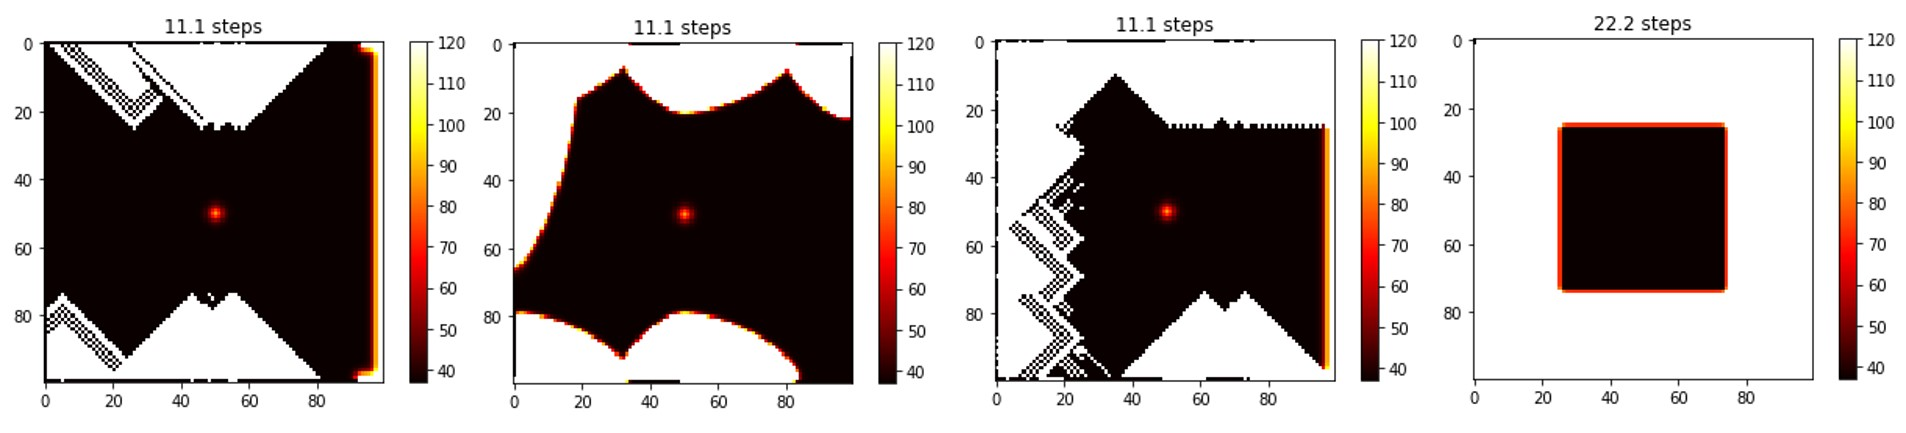
\includegraphics[width=0.95\linewidth]{Report_images/instability}
	\caption{Examples of instability caused by the perfusion term}
	\label{fig:instability}
\end{figure}

\subsubsection{2D model with added bone structures}	 	

Because of the difficulties with the perfusion term, when adding structure, we decided to consider first adding bones to the domain, so we could still use that the perfusion term is small. Initially we changed the constants

\begin{itemize}
	\item  Thermal conductivity
	\item  Thermal diffusion 
	\item  Specific heat capacity
	\item  Perfusion 
\end{itemize}

in a particular region of the domain to that for bone. The region can be seen on the left of figure \ref{fig:bone-without-changing-q}. The Gaussian source is focused at position $(50,50)$. 
On the right hand side of figure \ref{fig:bone-without-changing-q} you can see the results of the explicit method for this set up. As you can see,  there seems to be very little effect. In fact, looking at the values of the constants,  increase in the density of bone is offset by a decrease in the specific heat capacity of bone and decrease in thermal conductivity , comparing the constants in front of the diffusion term you see:  \begin{equation}
\frac{k_{muscle}}{\rho_{muscle} c_{muscle}} = \frac{0.5}{3430 \times 1041} \approx 1/7141260 \label{apples}
\end{equation}  and \begin{equation}
\frac{k_{bone}}{\rho_{bone} c_{bone}} =\frac{0.38}{ 1420 \times 1700} \approx 1/ 6352631. \label{bananas}
\end{equation}This is not a huge difference and it would take a long time for significant differences to be visible and running 1000 steps gave a residual of the difference between the bone and no bone simulations on the right of figure \ref{fig:bone-without-changing-q}. We are relieved to see there is a slight lack of symmetry with darker areas suggesting a greater change where the bone lies. However, the relative difference is still very small, less than a degree.

\begin{figure}
	\centering
	\includegraphics[width=\linewidth]{"Report_images/bone without changing Q"}
	\caption{Adding additional bone structure, varying thermal conductivity: thermal diffusion, specific heat capacity and perfusion constants but not varying Q. The left hand image shows the bone location, centre image the results of 1000 time steps and right most image the residual when we subtract the results with added bone from the results without added bone.  }
	\label{fig:bone-without-changing-q}
\end{figure}

We double check that the code is working correctly by  choosing the ``bone" to have a diffusivity constant of 10 times smaller than that of muscle. After 1000 steps this gives the results shown in figure \ref{fig:change-diffusion-constant}, which clearly shows a lack of symmetry and a slower diffusion process occurring in bone leading to lower temperatures in the bone. 

\begin{figure}
	\centering
	\includegraphics[width=0.8\linewidth]{"Report_images/change diffusion constant"}
	\caption{Experimenting with changing diffusion constant in a strip lying in the top half of the region, modelling bone}
	\label{fig:change-diffusion-constant}
\end{figure}

This was very unexpected compared to what is seen  experimentally. For example as discussed in paper \cite{Cochard2009}, by Caochard et al. they discuss how thermal ablation induced by high intensity focused ultrasound has produced promising clinical results to treat hepatocarcinoma and other liver tumours However skin burns have been reported due to the high absorption of ultrasonic energy by the ribs. They point to Duam et al. \cite{Daum1999}  in which it was reported that using magnetic resonance temperature monitoring of pigs in vivo that  temperature elevations were five times higher on the ribs than in the intercostal space. 

Looking back to the table in figure \ref{fig:tissueproperties} we see that we have yet to take into account the difference in the  attenuation coefficient in bone and in muscle. This would effect $ Q $, the source term in the equation and so we need to model this differently as the higher the attenuation coefficient the more energy absorbed by the ultrasound pulse and hence the higher $ Q $. 

  
 As a simple initial model, I multiplied the values of $ Q $ in areas of bone by a factor of $$ \frac{attenuation_{bone}}{attenuation_{muscle}} \approx \frac{105}{5} .$$
 
 Again, figure  \ref{fig:bone-with-changing-q} shows the location of the bone, the output of 1000 steps and  the residual of the code run without bone and the code run with bone. We can see that there is a clear asymmetry in the residual image - there is indeed greater heating in the bone.  However, we seem to have lost touch with reality in terms of temperature changes, with differences of about $ 4000 \degree C $ between the cases of bone and without bone. There is still some work needed to be done to get the form of Q correct. 
 
 \begin{figure}
 	\centering
 	\includegraphics[width=\linewidth]{"Report_images/bone with changing Q"}
 	\caption{Adding additional bone structure, varying thermal conductivity: thermal diffusion, specific heat capacity and perfusion constants and varying $ Q $ proportional to the attenuation constants in bone and in muscle. The left hand image shows the bone location, centre image the results of 1000 time steps and right most image the residual when we subtract the results with added bone from the results without added bone. }
 	\label{fig:bone-with-changing-q}
 \end{figure}
 


In order to experiment with changing structure and able to easily compare the effects of different structures I rewrote the semi-discretisation method as a class, with an input of the initial structure. Also instead of an explicit forward difference in time and central difference in time, used a Crank Nicholson method. 

We define the Crank Nicholson method in 1D as if $$ \frac{\partial u}{\partial t} = F\left(u,\, x,\, t,\, \frac{\partial u}{\partial x},\, \frac{\partial^2 u}{\partial x^2}\right)$$

then setting $u(i \Delta x,\, n \Delta t) = u_{i}^{n}\,$ we have: $$ \frac{u_{i}^{n + 1} - u_{i}^{n}}{\Delta t} = 
\frac{1}{2}\left[
F_{i}^{n + 1}\left(u,\, x,\, t,\, \frac{\partial u}{\partial x},\, \frac{\partial^2 u}{\partial x^2}\right) + 
F_{i}^{n}\left(u,\, x,\, t,\, \frac{\partial u}{\partial x},\, \frac{\partial^2 u}{\partial x^2}\right)
\right] \qquad $$

an implicit method. 

In our 2D case we ignore the perfusion term and use a small adaptation of the CN method using $T^i_{m,n}= T(i\delta t, m\delta x, n\delta y)$: $$F^i_{m,n} = \frac{1}{\rho c} \left( k\left[  \frac{(T^i_{m+1,n}-2T^i_{m,n}+T^i_{m-1,n})}{(\delta x)^2}+\frac{(T^i_{m,n+1}-2T^i_{m,n}+T^i_{m,n-1})}{(\delta y)^2}\right] +Q^i_{m,n}\right) $$
and \begin{equation}
\frac{T_{m,n}^{i + 1} - T_{m,n}^{i}}{\Delta t} = 
\left[
\lambda F^{i}_{m,n}+(1-\lambda)F^{i}+1_{m,n} 
\right] \qquad \label{method}
\end{equation} 

Where $ \lambda =\frac{1}{2} $ gives the Crank Nicholson method, $ \lambda =1 $ gives a completely explicit method and $ \lambda=0.55 $ gives a good balance between stability and accuracy. 

Implementation can be quite costly. I have coded it  on a $ M\times M  $ grid, where for each time step, the grid of temperatures is written as a length $ M^2 $ vector, say $V$,  and then two matrices are formulated such that: $$ A_1 V^{i+1}=A_2 V^{i}.$$ Inverting $A_1$, a $M^2\times M^2$ matrix can be costly  but the matrix is sparse and Toeplitz so the matrix operations can be optimised. 

Alternatively, for $\lambda=0.5$ we could use the alternating direction implicit method which is designed for 2D methods, in  which the iteration process alternately updates the column and row spaces of approximate solutions, restricting all matrices to size $M \times M$.

Interestingly, the size of $M$ seems to be vital for stability. For time steps of just 0.005 then a maximum of $M=25$ is possible for the ADI method where as for the method in equation \ref{method} with $ \lambda=0.55 $,  $M$ can be larger, but instability occurs around $ M=40 $, although much above this computational time becomes prohibitive anyway. 

In figure \ref{fig:various-bone-structures}  I give examples of different bone configurations and the results of method in equation  \ref{method} with $ \lambda=0.55 $. You can clearly see that bone is being heated much more strongly than muscle tissue by the source and there is some evidence of larger diffusion in muscle tissue although as we saw in calculations \ref{apples} and \ref{bananas} this effect is quite small and more iterations would be required to really see these effects. 

\begin{figure}
	\centering
	\includegraphics[height=0.8\textheight]{"Report_images/various bone structures"}
	\caption{Implementation of the method in equation  \ref{method} with $ \lambda=0.55 $ for varying bone structures. The bone structure is given on the left (note that anything non-zero i.e. not dark blue is taken to be bone) with results of only a few iterations on the right hand side( More iterations would have been more computationally intensive). In all case the focus of the source is at the point (20,20). }
	\label{fig:various-bone-structures}
\end{figure}



\subsection{Case Study Conclusions and Next Steps}

To conclude this case study it is worth discussing if what we have so far is useful, what possible next steps there might be - both immediate and long term and finally what I have learnt from such an in depth study of a study group problem. 

What we have so far, is a very basic 2D model of heat transfer in a medium that potentially has some structure or inhomogeneities. The structure can be easily changed to model different scenarios  or rotations and the model runs relatively quickly an a university desktop. In its current state it is a long way from something that could model the complexities of the human body, however there are clear avenues for improvement and these include: 

\begin{itemize}
	\item More accurate modelling of $ Q $, such as that seen in paper \cite{Scott2014} and in equation \ref{ComplicatedQ}. Varying the exponential factor based on the ultrasound attenuation coefficient of the media will be a quick but not computationally expensive way of adding accuracy. 
	\item Add the perfusion terms back into the Crank Nicholson models and investigate stability. Potentially then, we could look at cases with large blood vessels when perfusion will play a much greater effect
	\item A greater handle on units and on length scales would be useful to get a clearer understanding of how the model relates to reality and to ensure that thermal dose measurements produce sensible values. In most cases, I think that we have got there on temperature changes, with temperature values mimicking those that might be seen experimentally: this is an improvement on the study group code that was plotting a temperature profile, that didn't have a clear link to reality.  Length and time scales, however,  are still uncertain. This should not be a difficult but may be a long job.
	\item A long term goal would be the production of a  3D model. This would enable us  to look at examples such as the skull, rib cages or the spinal chord where bone encompasses the region of interest. It would also allow us to look at realistic structures of multiple bones that could possibly effect the area of heating.
\end{itemize}

Reflecting on this case study as a piece of industrial mathematics, we can see that it has the potential for high impact. A realistic model would reduce the need to experiment on animals with a certain amount of the trial and error able to be tested on the model. It could also be used before a procedure, to see if treatment might be viable or test different approaches. This could improve treatment outcomes. It is also a modelling problem best approached by a mathematician, the issue of the perfusion term causing instability in standard numerical models will require careful handling. The main takeaway, I think, is the interdisciplinary nature of this project, touching most many areas of mathematics, physics, biology and engineering. It highlights the need for industrial mathematicians to be curious about many areas, adaptable and able to work with a a part of a large interdisciplinary team. I think that if this project were to be taken any further, effort should be made to bring in expertise from medicine, physics and engineering to guide and enrich the project. 
  \pagebreak
	\section{Final Thoughts} 
In this reading course, although short, I spent some time exploring the breadth of what encompasses Industrial Mathematics.  I had thought I understood the importance of Mathematics to many aspects of daily life and social and economic innovation but I still found myself surprised by some applications, getting lost in papers on everything from  Maple Tree Sap \cite{Stockie2015} to real-time face detection \cite{Viola2004}. Talking to non-mathematical, although highly educated, friends and family they have also been surprised by some of the topics I have been researching. Somehow I think that mathematics needs a public relations re-brand, people imagine large calculations, endless bits of paper and dusty books they don't think about the AI in their new smart-phone, the security of their internet purchases, the latest vaccination program or the milk they can by late evening on a Sunday in the local shop. With greater awareness will come talented individuals, more funding and more opportunities for collaboration. 


The extended case study on High Intensity Focused Ultrasound demonstrated clearly the interdisciplinary nature of industrial mathematics. Mathematical modelling was based on the physics of the heat equation, the  wave physics of attenuation and absorption and propagation and imaging relying on phase changes. Construction and focusing of the ultrasound relies heavily on very precise engineering and obviously things are going on in the very complex human body, and a biological perspective is necessary. It highlights how flexible industrial mathematicians need to be approaching a problem, needing to change perspectives, take on new material and explain complex concepts to non-mathematicians. 
There is the potential for future work on a more flexible 3D model for modelling heat transfer due to HIFU in the body though if an extended piece of research were to be attempted a deeper literature review would need to be done and I think a reconnection with those directly using and developing HIFU would be valuable to focus research objectives and get a clear direction of the movement of the field. 

To conclude, I considered three areas of improvement for the future of Industrial Mathematics. A warning however, that  I am certainly biased. I am at the point of choosing a subject of a mathematics PhD and looking for a career in which I can use and expand my mathematical knowledge, embark on research and do some social and economic good. 

For my first area, I think that a big emphasis needs to be on developing clear career pathways and opportunities for early career researchers. They need to include a competitive package and terms to compete with industry and there needs to be flexibility to move to and from industry recognizing the skills and connections that this brings to a department on par with publishing output. I see some good examples such as CASE PhD projects or  Commercial Research Associates at the Institute for Mathematical Innovation but not clear options for progression in this type of industrial research. 

Secondly, I return to my comments on undergraduate placements, internships and years-in-industry. I urge both academic institutions and industry to work together when setting up projects, to ensure that students get a clear idea of the nature of research: reading papers, getting stuck, trying new things, getting stuck, presenting their results to peers and experts, preparing reports and much more. Producing ``code monkeys" is all very well, but what would be better is to equip mathematical graduates with the problem solving skills, determination and communication skills to make excellent researchers in academia or in industry. The increase in CDTs is a great move in training the next generation of researchers, but only a small minority of mathematics undergraduates go on to pursue a PhD. 

Finally, I come to one recommendation made by the Bond report \cite{Bond} that I am yet to mention but support wholeheartedly: ``Awareness should be raised within the mathematical sciences community of wider research challenges and societal challenges (including the sustainable development goals"). With a vast talent pool but limited resources, focusing an the most important challenges is vital. As we have seen the Research Councils' and Higher Education Funding Councils' are increasing their emphasis on research impacts but there is a individual researchers must also take some responsibility.
 
\pagebreak	
	\bibliography{Industrial_Reading_Project}
	\bibliographystyle{plain}
\end{document}